% this file is called up by thesis.tex content in this file will be fed into the
% main document

% : ----------------------- name of chapter  -------------------------
\chapter{Planning Constant-Depth Paths under AUV Motion Constraints}
\label{ch:motion_constratins}
% top level followed by section, subsection


% : ----------------------- paths to graphics ------------------------

% change according to folder and file names
\ifpdf
    \graphicspath{{3_motion_constraints/figures/PNG/}{3_motion_constraints/figures/PDF/}{3_motion_constraints/figures/}}
\else
    \graphicspath{{3_motion_constraints/figures/EPS/}{3_motion_constraints/figures/}}
\fi

% : ----------------------- contents from here ------------------------

% As explained in Section~\ref{sec:motion_constraints_review}, planning problems
% for robotic systems can be categorized in one of the two groups:
% \begin{inparaenum}[1)] \item path planning, which refers to those problems that
% only consider geometric constraints, and \item motion planning for those that
% also consider the kinematic and/or dynamic aspects of the system.
% \end{inparaenum}
% However, some authors use the latter term to refer to either
% group~\cite{Sucan2011},~\cite{LaValle2006}. Throughout this thesis, both terms
% are used interchangeably, nonetheless there will be a special emphasis when
% referring to the motion constraints involved, since they have been a determining
% aspect in meeting the proposed objectives.

Recent and potential applications for \acp{AUV} mentioned in
Chapter~\ref{ch:introduction} establish most of the motion planner requirements,
such as online computation, motion in \ac{3D} workspaces, and navigation along
unexplored environments in close-proximity to nearby obstacles. All these
constraints can be met with sampling-based planning methods. Particularly for
navigating in close-proximity, one desired characteristic is being able to
calculate feasible motions that take into account the \ac{AUV}
capabilities. This allows minimizing unexpected vehicle trajectories when
attempting to follow the calculated path. In this respect, this chapter firstly
explains the equations of motion used to approximate the \ac{2D} (at a constant
depth) vehicle behavior for motion-planning purposes. Secondly, it explains two
different approaches to integrate such equations into the motion planner.
Lastly, it presents and discusses the results obtained with both approaches in a
simulated environment.

\section{2D First-Order Motion Model}
\label{sec:2d_kinematic_model}

As occurs with any mechanical system, \ac{AUV} motions can be formulated with
kinematic and dynamic models. The former ones describe the geometry of motion by
relating the system positions and velocities. Dynamic models, on the other
hand, not only include the system kinematics, but also take into account the
forces and torques that generate the motions. This latter kind of model is
generally employed for designing robust controllers, however, their high
computational cost makes them an inappropriate approach for the scenarios
proposed in this thesis, which require an online (re)planning behavior. The
associated overhead is especially true when using sampling-based planning
methods, where all configurations are generated by evolving the system, \ie
performing numerical integration of the equation of motion. Alternatively, a
kinematic model provides a less accurate approximation for the vehicle's motion
constraints, but it also allows additional computation time that can be
dedicated to finding better collision-free paths.

In order to establish which kinematic model must be used, it is necessary to
understand the vehicle motion capabilities and the possible test scenarios. In
some \ac{AUV} applications, a first valid approximation is to assume that the
vehicle navigates at a constant depth (see
Sec.~\ref{sec:StateOfTheArtPlannAUV}). Furthermore, if the vehicle is a
torpedo-shaped \ac{AUV}, usually, it will only be able to changing its direction
of motion by moving forward/backward. In the case of the Sparus~II \ac{AUV}, the
vehicle is equipped with two back thrusters that allow it to spin over. However,
it is still not capable of conducting lateral motion. Therefore, it is correct
to affirm that the vehicle is subject to a motion constraint along its y-axis
(see Fig.~\ref{fig:RefFramesAUV2D}).

As explained in Chapter~\ref{ch:introduction}, motion or differential
constraints can be expressed as a set of differential equations in the general
form $\dot{q}=f\left(q,u\right)$, where $q$ and $\dot{q}$ are the system state
and its first derivative, respectively, and $u$ is the control input.
Having this in mind, and considering the aforementioned constraints when
navigating at a constant depth, a non-holonomic and torpedo-shaped \ac{AUV} can
be represented as a simple car-like vehicle, with a first-order motion model
defined as follows:

\begin{equation}
\label{eq:KinEqAUV2D}
	\begin{bmatrix}
		\dot{x}\\
		\dot{y}\\
		\dot{\psi}\\
	\end{bmatrix}=
	\begin{bmatrix}
		v\ cos\left(\psi\right) \\
		v\ sin\left(\psi\right)\\
		w\\
	\end{bmatrix}
	\text{,}
\end{equation}

where $q=\left[x, y, \psi\right]^T$ corresponds to the system state that
includes its \ac{2D} position and orientation with respect to an inertial
reference frame, and $\dot{q}=\left[\dot{x}, \dot{y}, \dot{\psi}\right]^T$ is
the first time derivative that depends on the state itself and the control
inputs, \ie linear/surge speed ($v$) and turning rate ($w$). From
Eq.~\eqref{eq:KinEqAUV2D}, it can be concluded that the \ac{C-Space} of a
torpedo-shaped \ac{AUV} is $\mathcal{C} = SE(2) = \mathbb{R}^2 \times SO(2) =
\mathbb{R}^2 \times \mathcal{S}$. Figure~\ref{fig:RefFramesAUV2D} depicts the
inertial frame, the body-fixed frame, and the different variables (positions and
velocities) contained in~\eqref{eq:KinEqAUV2D}.

\begin{figure}[htbp]
	\centering
	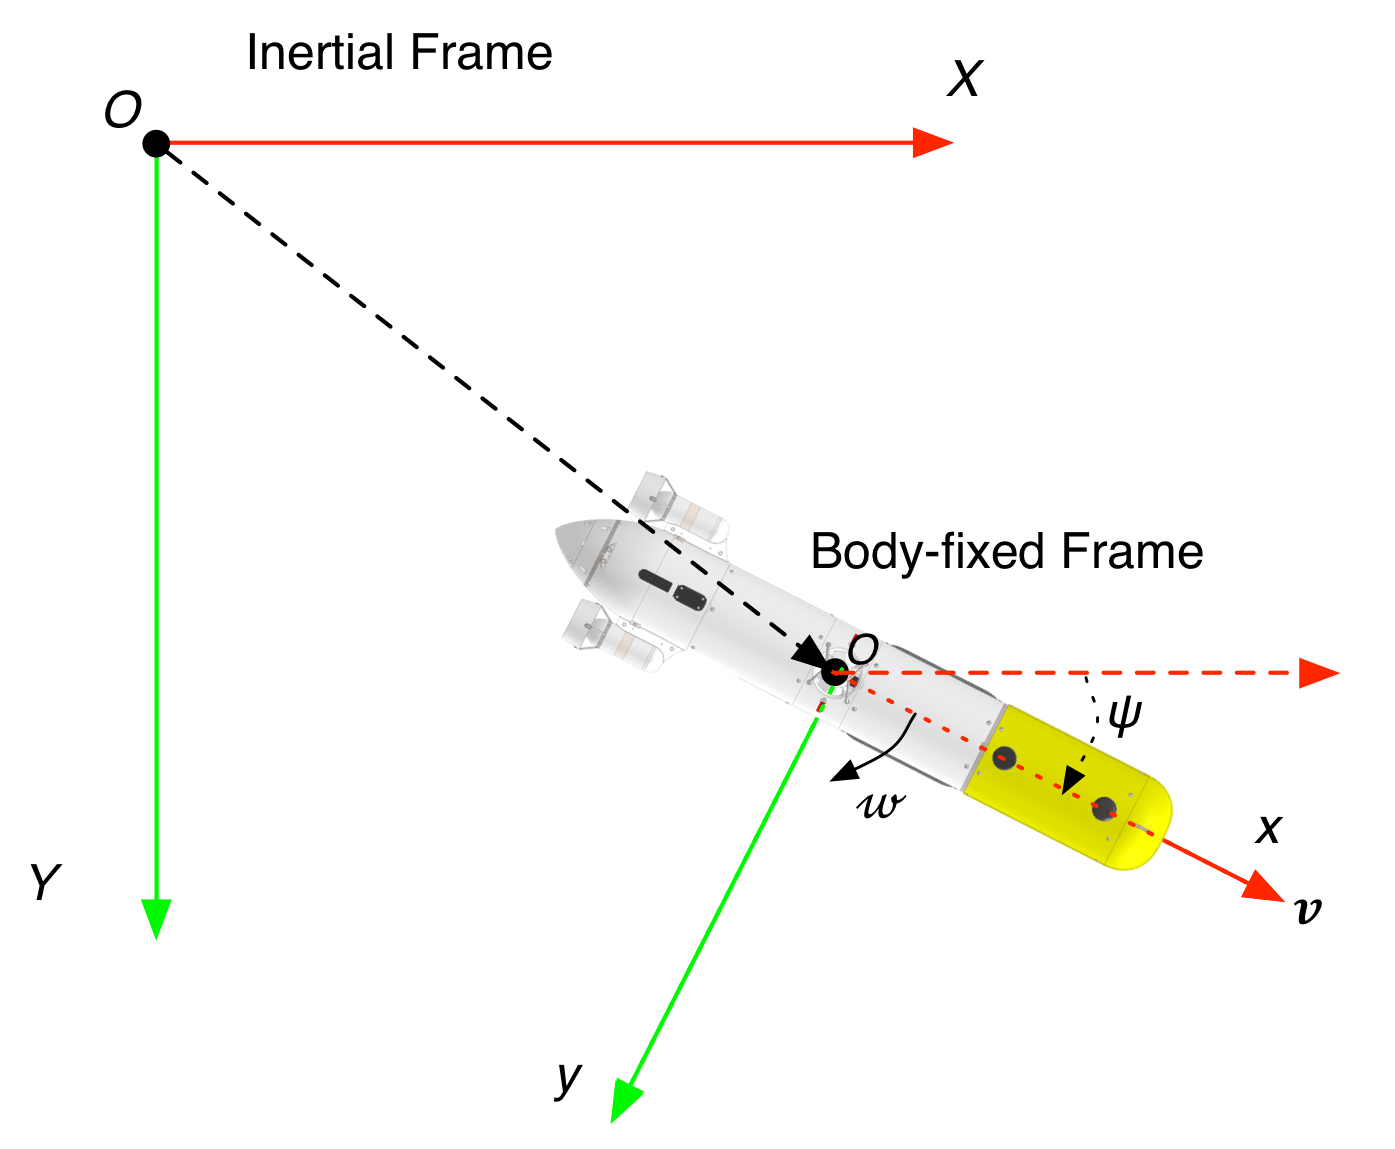
\includegraphics[width=.7\linewidth]{RefFramesAUV2D} \quad
	\caption[Top view of the Sparus~II AUV, including the inertial and body-fixed
	frames, and the 2D vehicle state and control variables.]
	{Top view of the Sparus~II AUV, including the inertial and body-fixed
	frames, and the 2D vehicle state and control variables.}
	\label{fig:RefFramesAUV2D}
\end{figure}

Once the constraints have been established through the corresponding
differential equations, the next step is to define an appropriate strategy to
generate feasible motions that meet such constraints. The following
sections present two different approaches, which use sampling-based algorithms
to calculate such kind of motions for a torpedo-shaped \ac{AUV} that navigates
at a constant depth.

\section{Motion Planning by Using Differential Equations}
\label{sec:expan_2d_diff_eq}

% Although some of the classical grid-based methods have addressed the problem of
% planning motions under differential constraints (see
% Sec.~\ref{sec:motion_constraints_review}), those approaches establish a grid
% over the \ac{C-Space} and define a finite set of possible maneuvers, thus
% reducing the number of viable solutions. On the other hand, 
Sampling-based algorithms, especially the \ac{RRT}~\cite{LaValle2001} and its
variants, have proved to efficiently explore the \ac{C-Space} while taking all
the motion constraints into account. Furthermore, there are other
characteristics such as the incremental search behavior, which allows these
methods to continuously (re)plan the solution path as the vehicle moves through
unexplored environments (see Chapter~\ref{ch:plann_online}). All this together
makes an \ac{RRT}-based algorithm the appropriate approach for the intended
\ac{AUV} applications.

As explained in Section~\ref{sec:RRT}, the \ac{RRT} algorithm builds a single
tree that is rooted at an initial state (configuration), which is incrementally
expanded towards uniformly randomly \textit{sampled} states\footnote{There
exists another RRT variant called RRT-Connect that grows two trees, one from the
start state and another one from the goal state. However, this is not possible
when dealing with motion constraints, since merging both trees at a common
configuration may become computationally intractable~\cite{Kuffner2000}.}. This
procedure is the same as the one initially presented in
Algorithm~\ref{alg:SampleRRT}, being this a particular case where a random state
corresponds to $q_{rand}\in SE(2)$, as explained before. In order to
\textit{extend} the tree towards $q_{rand}$ while meeting the vehicle's motion
constraints, new collision-free motions (states) are obtained by integrating the
vehicle's equation of motion, such as Eq.~\eqref{eq:KinEqAUV2D}. In such a case,
instead of using Algorithm~\ref{alg:ExtendRRT}, the tree expansion can be
rewritten as shown in Algorithm~\ref{alg:ExtendRRTDiffConstr}. This procedure
firstly requires finding the state $q_{near}$, that is the nearest to $q_{rand}$
(line~\ref{alg_line:findNearest}). This can be done by using a weighted metric
to calculate the distance between configurations. Such a metric combines the
translation component, calculated as the Euclidean distance, and the orientation
component, calculated as the smallest orientation
difference~\cite{Choset2005,LaValle2006}.

\begin{algorithm}[htbp]
\DontPrintSemicolon

	\SetKwFunction{calcNewState}{calcNewState}
	\SetKwFunction{findNearestNeighbor}{findNearestNeighbor}
	\SetKwFunction{addNewNode}{addNewNode}
	\SetKwFunction{addNewEdge}{addNewEdge}
	\SetKwFunction{findInput}{findInput}
	
	\KwIn{\\ 
	$T$: tree of collision-free configurations.\\ 
	$q_{rand}$: configuration towards which the tree will be extended.\\
 	$\mathcal{C}$: \ac{C-Space}.}
	\KwOut{\\ Result after attempting to extend.}
	\Begin{
	 	$q_{near}\leftarrow T.$\findNearestNeighbor{$q_{rand}$}\;\label{alg_line:findNearest}
	 	$u_{near\_ to\_rand}\leftarrow$\findInput{$T,q_{near},q_{rand}$}\;\label{alg_line:findInput}
	 	$q_{new}, collision\leftarrow$\calcNewState{$q_{near},u_{near\_to\_rand},\Delta t$}\;\label{alg_line:calNewState}
	 	\If{$collision = FALSE$} {\label{alg_line:ifCollision} 
	 		V.\addNewNode{$q_{new}$}\;
	 		E.\addNewEdge{$q_{near},q_{new}$}\;\label{alg_line:addNewEdge}
	 	}
 	}
\caption[extendRRT when dealing with motion constraints.]
{extendRRT (when dealing with motion constraints)}
\label{alg:ExtendRRTDiffConstr}
\end{algorithm}

Once the nearest motion has been found in the tree, the next step is to
calculate the control input $u_{near\_ to\_rand}=\left[v, w\right]$ that has to
be applied in order to change the vehicle state from $q_{near}$ towards
$q_{rand}$ (line~\ref{alg_line:findInput}). With an \ac{RRT} algorithm under
geometric constraints the tree is iteratively expanded a geometric distance
$\epsilon$ (see Algorithm~\ref{alg:ExtendRRT},
line~\ref{alg_line:ExtendRRTGeom}), in the case of an \ac{RRT} algorithm under
motion constraints the tree is expanded by applying an input $u$ for a period of
time $\Delta t$ (line~\ref{alg_line:calNewState}).

In some \ac{AUV} applications, a common assumption is that the vehicle navigates
at a constant surge speed $v$, but can vary its turning rate $w$ up to a maximum
value $w_{max}$. This means that calculating the input $u$ is limited to firstly
establishing a constant $v$ that will be used along the mission, and then
computing a valid value for $w$ that meets the vehicle motion constraints. There
are different approaches that permit calculating $u$. Two alternatives, also
presented by LaValle and Kuffner~\cite{LaValle2001}, are either to randomly
sample the control space, or to test a number of possible inputs and then select
the one that generates the state $q_{new}$ that is closest to $q_{rand}$. The
implementation used in a first stage of this thesis is based on a combination of
both approaches.

In such an implementation, instead of testing a large number of different
turning rates $w$, a set of five possible values is established as
follows: $w_{control_i} \in \left\{-w_{max}, -\frac{w_{max}}{2}, 0,
\frac{w_{max}}{2}, w_{max}\right\}$. These values, in turn, define a
set of four sub-intervals over the control space:
%
$\{[-w_{max}, -\frac{w_{max}}{2}],$ $[-\frac{w_{max}}{2}, 0],
[0, \frac{w_{max}}{2}], [\frac{w_{max}}{2}, w_{max}]\}$.
%
Then, using Eq.~\eqref{eq:KinEqAUV2D} with $q_{near}$ as the starting state, each
$u_i = \left[v, w_{control_i}\right]$ is applied for a period of time $\Delta t$
to generate five different states $q_{control_i}$. Having them, it is possible
to estimate which of the four sub-intervals may contain a control input that
leads the tree expansion from $q_{near}$ closer to $q_{rand}$. The final value
of $w_{rand}$ is obtained by sampling a random turning rate over the chosen
sub-interval. This procedure avoids discretizing the control space, which would
imply the loss of the random exploration of the \ac{C-Space}, an important
property of the original algorithm. Figure~\ref{fig:ControlInputSampling}
presents the main concept of the control input selection.

\begin{figure}[htbp]
	\centering
	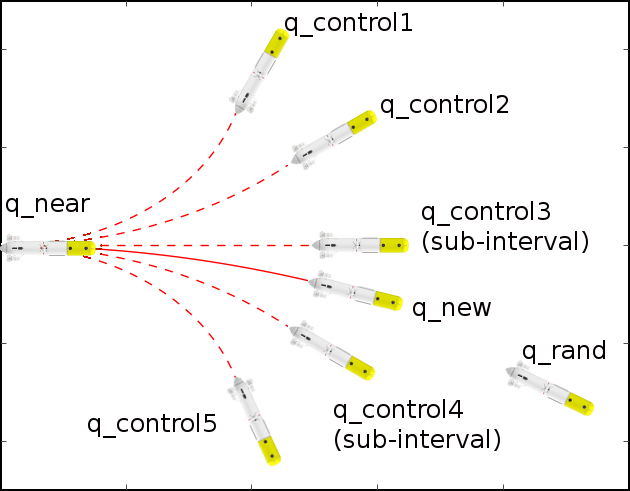
\includegraphics[width=.6\linewidth]{ControlInputSampling} \quad
	\caption[Control input selection for expanding an RRT under the differential
	equation.]
	{Control input selection. Tree is expanded from $q_{near}$ towards
	$q_{rand}$. To do so, an interval of possible turning rates ($q_{control\_i}$)
	are evaluated. This permits defining a sub-interval from which the control
	input is sampled randomly, and is applied to generate the new state
	$q_{new}$.}
	\label{fig:ControlInputSampling}
\end{figure}

The remaining of the \textit{extend} procedure
(Algorithm~\ref{alg:ExtendRRTDiffConstr}) calculates the new state $q_{new}$
(line~\ref{alg_line:calNewState}). This is done by integrating
Equation~\eqref{eq:KinEqAUV2D} while using the final sampled input $u_{near\_
to\_rand} = \left[v, w_{rand}\right]$. Finally, if $q_{new}$ is proved to be
collision-free, it is added and connected to the tree
(lines~\ref{alg_line:ifCollision}-\ref{alg_line:addNewEdge}).
Figure~\ref{fig:RRTDiffConstr} depicts an example of an \ac{RRT} algorithm that
solves a start-to-goal query under these motion constraints.

\begin{figure}[htbp]
    \myfloatalign
    \subfloat[]
    {\label{fig:RRTDiffConstrStep1}
    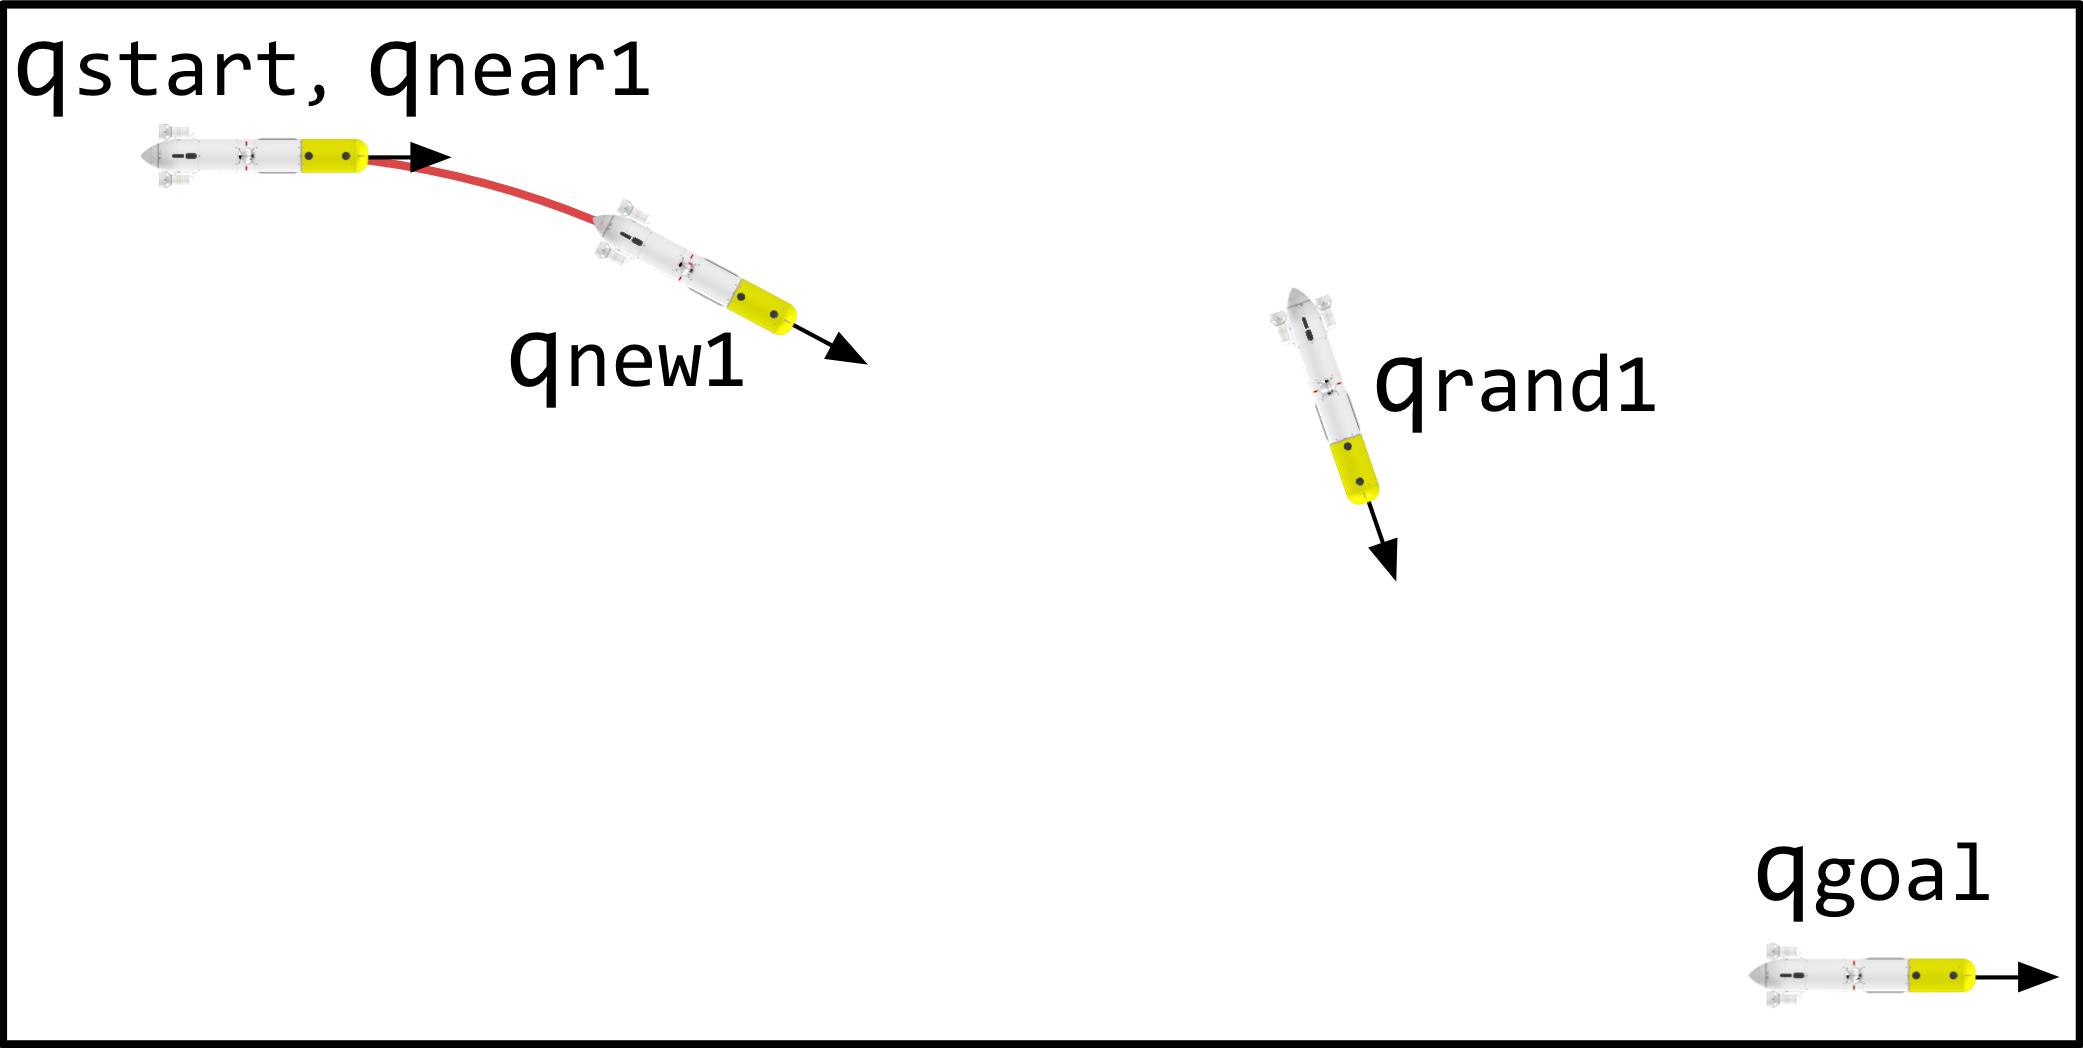
\includegraphics[width=.42\linewidth]{ExpansionRRTDiff-a}} \quad
    \subfloat[]
    {\label{fig:RRTDiffConstrStepi}%
     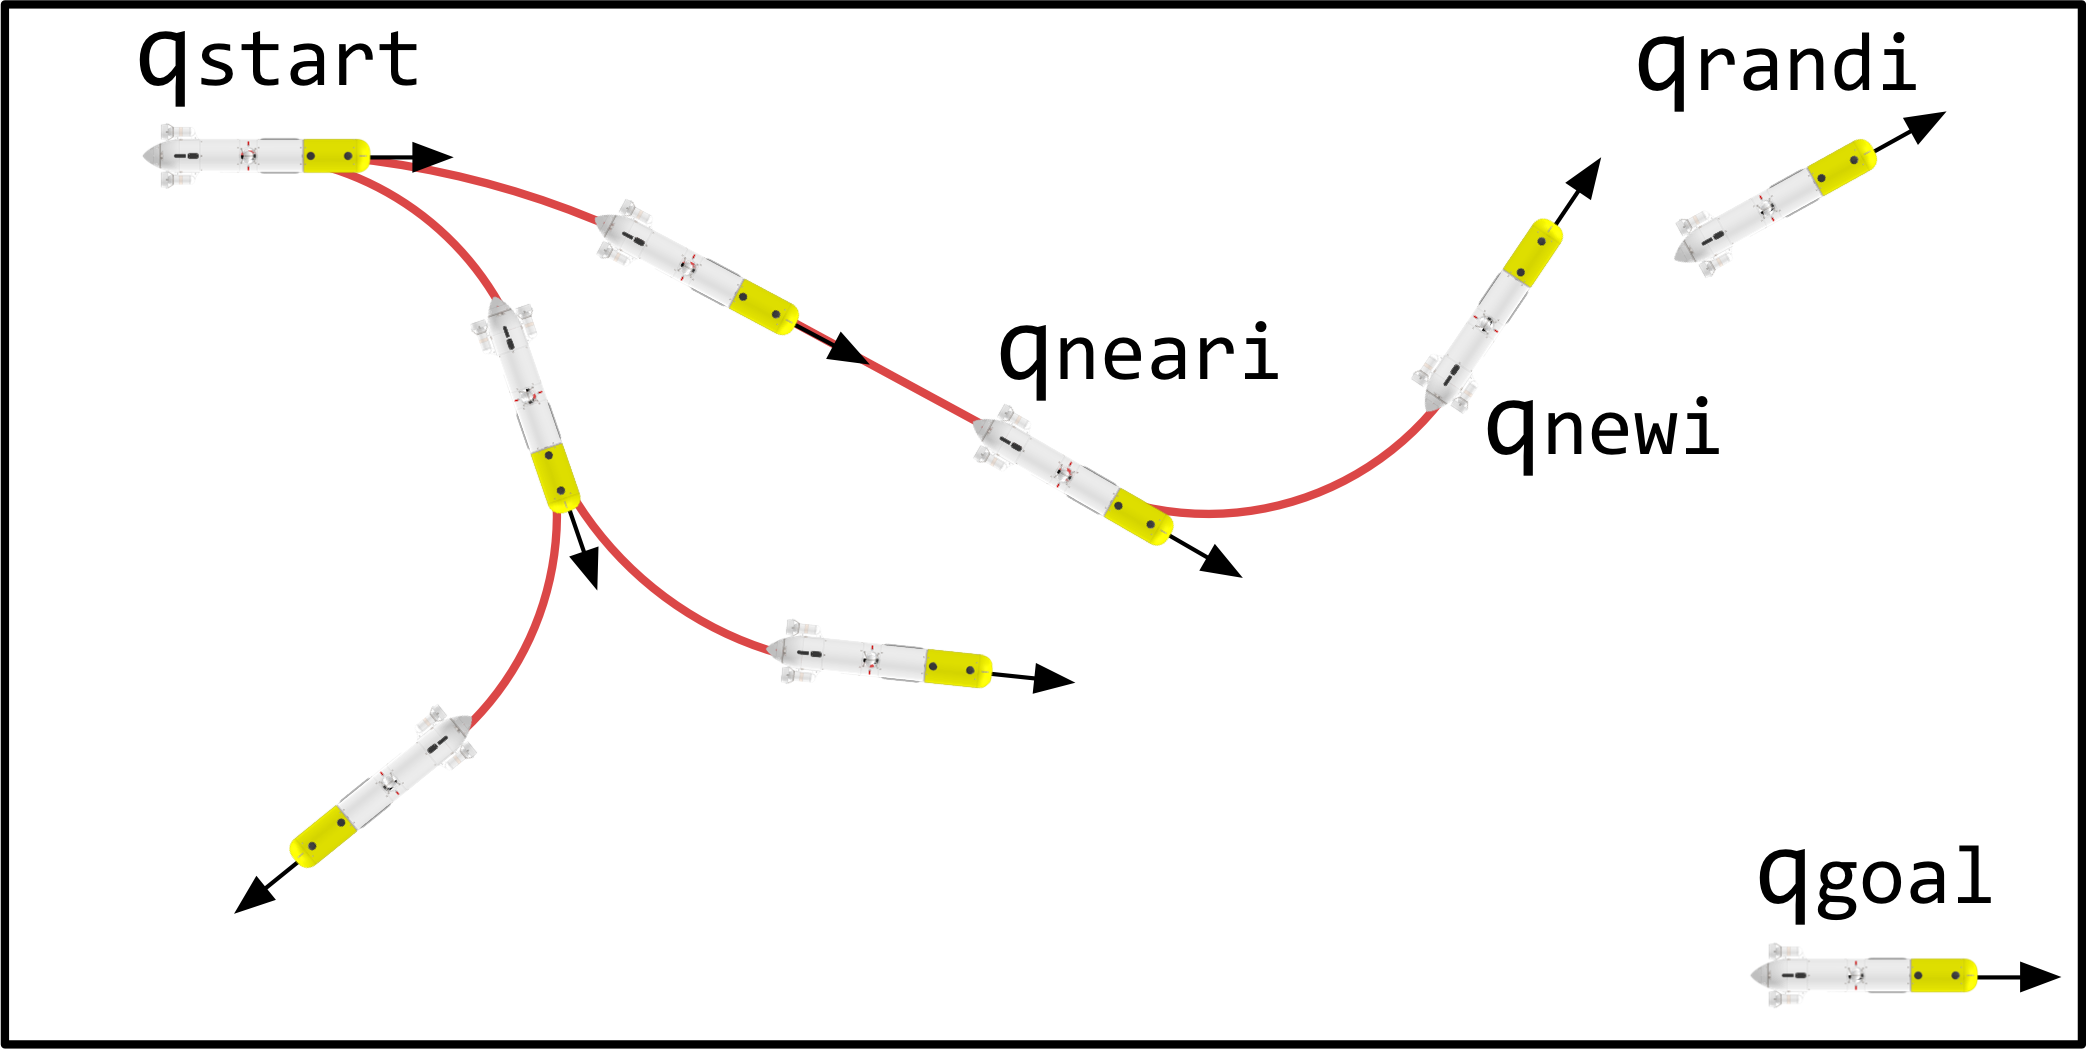
\includegraphics[width=.42\linewidth]{ExpansionRRTDiff-b}} \quad
    \subfloat[]
    {\label{fig:RRTDiffConstrComplete}
    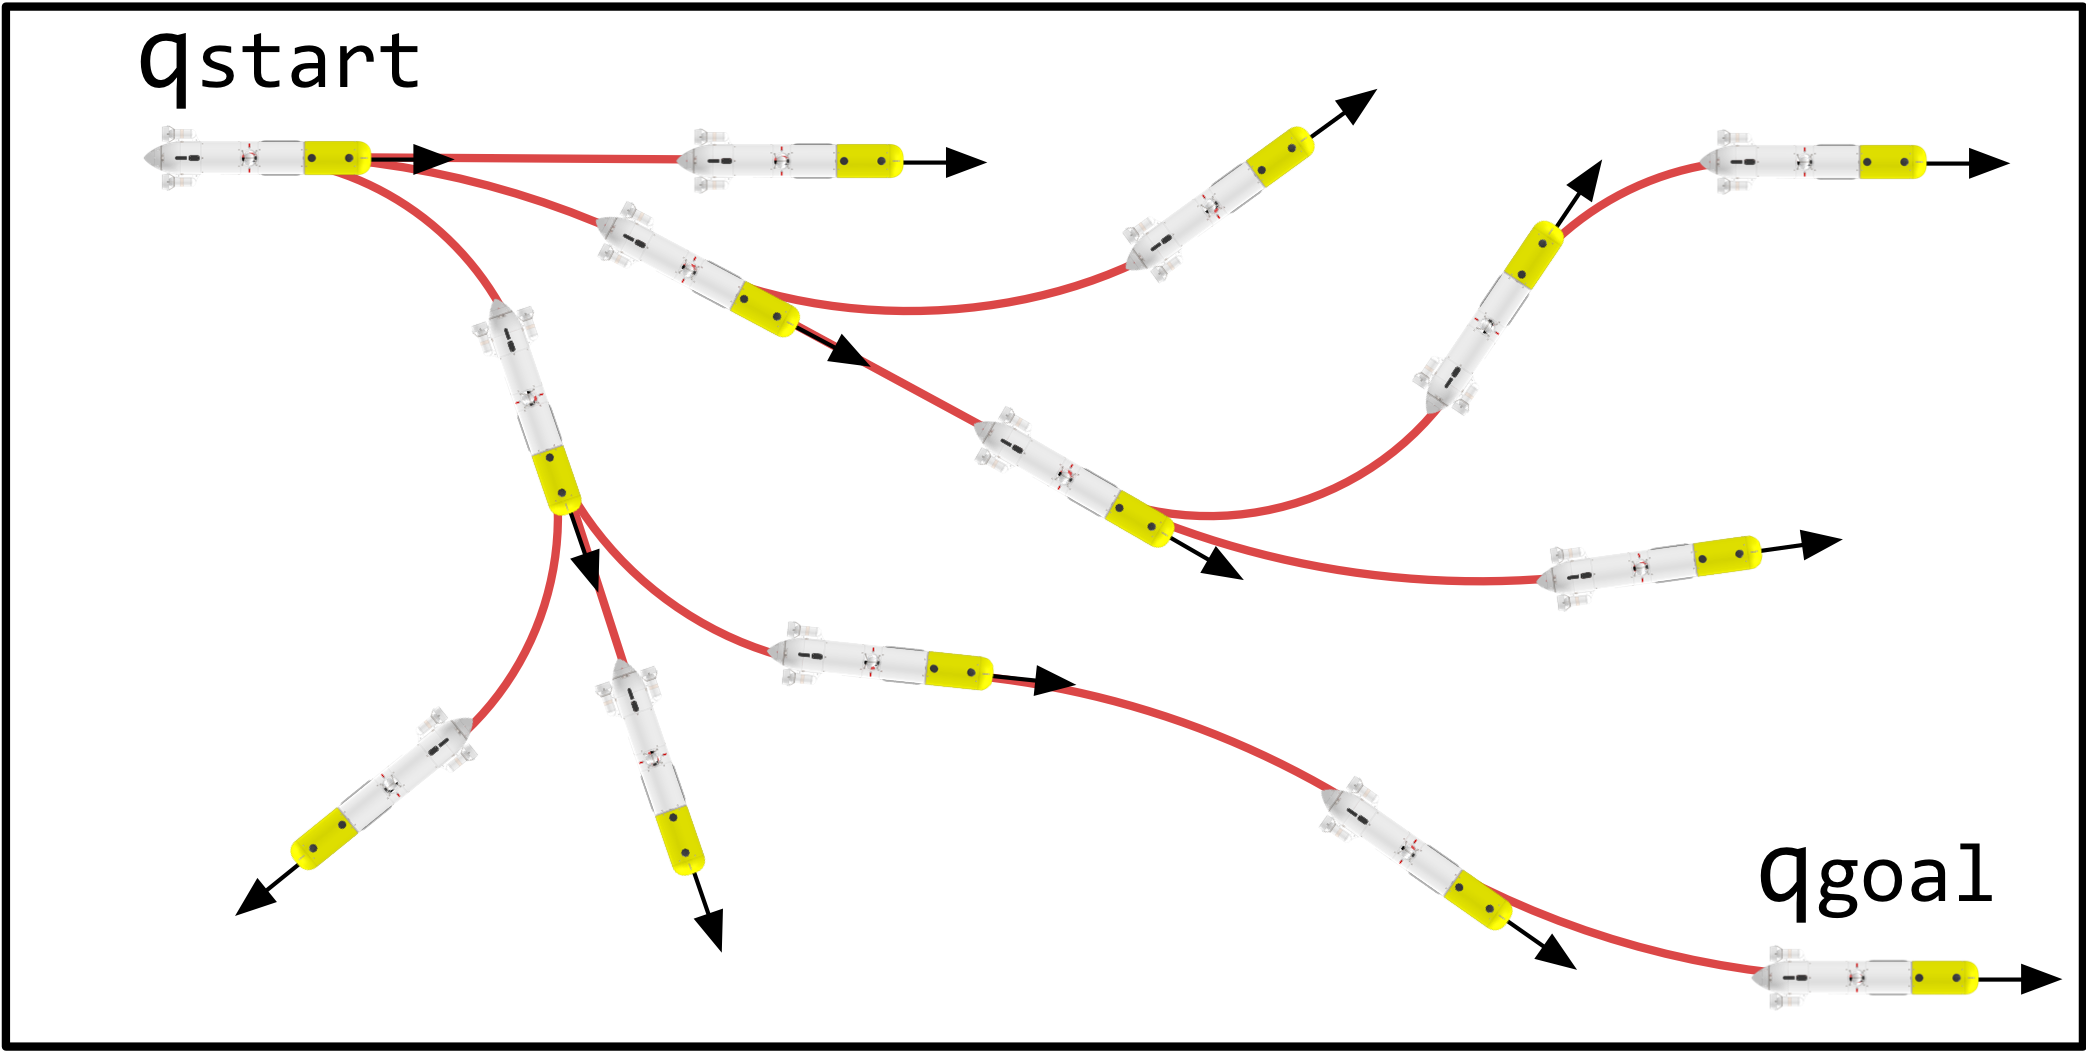
\includegraphics[width=.42\linewidth]{ExpansionRRTDiff-c}}
\caption[Start-to-goal query solution by expanding an RRT algorithm that
considers the differential constraints of a car-like system.]
{Tree expansion of an \ac{RRT} algorithm that considers the differential
constraints described by Equation~\eqref{eq:KinEqAUV2D}.
\protect \subref{fig:RRTDiffConstrStep1} Given the start and goal states, a
first random sample is used to generate the first expansion of the tree
($q_{new}$).
\protect \subref{fig:RRTDiffConstrStepi} The expansion $i^{th}$ of the tree.
\protect \subref{fig:RRTDiffConstrComplete} A feasible path has been found from
the start to the goal state.}
\label{fig:RRTDiffConstr}
\end{figure}

%\cleardoublepage

\section{Motion Planning by Using Dubins Curves}
\label{sec:expan_2d_dubins}

There are several examples where a purely geometric path is first computed, and
then it is transformed into a path that is appropriate for the considered
vehicle. For example, Yang \etal used an \ac{RRT} algorithm to find a route of
collision-free waypoints, which is interpolated with a cubic B\'ezier
spiral~\cite{Yang2008}. This seeks to convert the initial route into a smooth
and feasible path for an \ac{UAV}. As another example, Kuwata \etal proposed to
expand an \ac{RRT} by considering not only the vehicle dynamics, but also its
controller behavior~\cite{Kuwata2009}.

There are other \ac{RRT}-based approaches that have been proposed to generate
feasible paths for aerial and terrestrial vehicles. In one of those approaches,
for instance, a geometric \ac{RRT} algorithm finds a route of collision-free
waypoints, which are interpolated with a cubic B\'ezier spiral. This seeks to
convert the initial route into a smooth and feasible path for an
\ac{UAV}~\cite{Yang2008}. In another approach that is closer to the one
presented in the previous section, an \ac{RRT} algorithm is expanded by
considering not only the vehicle dynamics, but also its controller
behavior~\cite{Kuwata2009}.

Nonetheless, all those approaches, including the one presented in the previous
section, have a major drawback; they do not guarantee optimality for any metric.
It is a common characteristic of most sampling-based methods, at least in their
original form. This issue could be critical in underwater applications, which
may require optimizing different criteria such as visibility (for gathering
information), vehicle autonomy, or even the safety associated with a path when
navigating in close-proximity to nearby obstacles.

As explained in Section~\ref{sec:SamplOptimalPlan}, one option to cope with this
situation is to use the \ac{RRT*} algorithm, which is a variant that
incorporates the asymptotic optimality property~\cite{Karaman2011}.
Its main difference with respect to other \ac{RRT}-based methods, is a routine
that checks if reconnecting new state's nearest nodes improves their associated
cost. This implies that the probability of obtaining an optimal path converges
to 1 over time. (see Algorithm~\ref{alg:ExtendRRTstar}). For doing this, the
\ac{RRT*} algorithm requires a steering function that permits calculating such
states (nodes) reconnection. In the case of systems under motion constraints,
having such a function implies calculating the required input to dynamically
evolve the system from a given state to a desired one. However, defining this
function requires solving a two-point boundary value problem, which is in
general a very difficult problem.

For the purposes of this thesis, as an alternative to defining a steering
function, it is possible to adopt the Dubins vehicle model~\cite{Dubins1957}.
Dubins geometrically demonstrated that, for a system that is only capable of
traveling forward and with a constraint on the curvature of the path, the
shortest path to connect any two configurations (states) $q_i,q_j \in SE(2)$,
when no obstacles are present, can be obtained analytically by the combination
of circular arcs and straight lines. Using three possible maneuvers as input,
left (L), straight (S) or right (R), Dubins curves define six possible
combinations: RSR, RSL, LSR, LSL, RLR, LRL. For a Dubins vehicle, at least one
of these characterizes the optimal (shortest) trajectory between two states (see
Fig.~\ref{fig:DubinsPathsExample}).

\begin{figure}[htbp]
    \myfloatalign
    \subfloat[RSL]
    {\label{fig:DubinsRSL}
    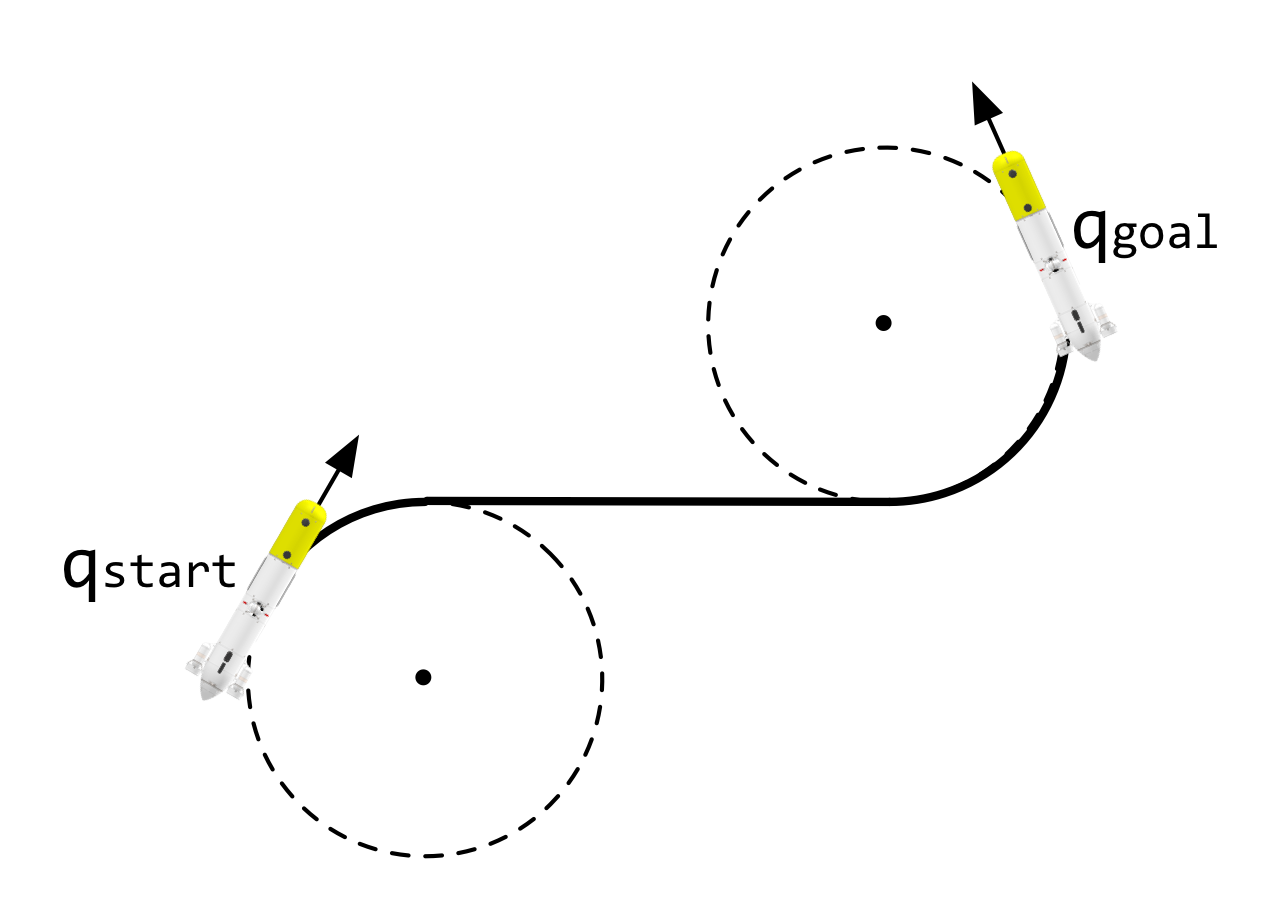
\includegraphics[width=.45\linewidth]{DubinsRSL}} \quad
%     \subfloat[RSR]
%     {\label{fig:DubinsRSR}%
%      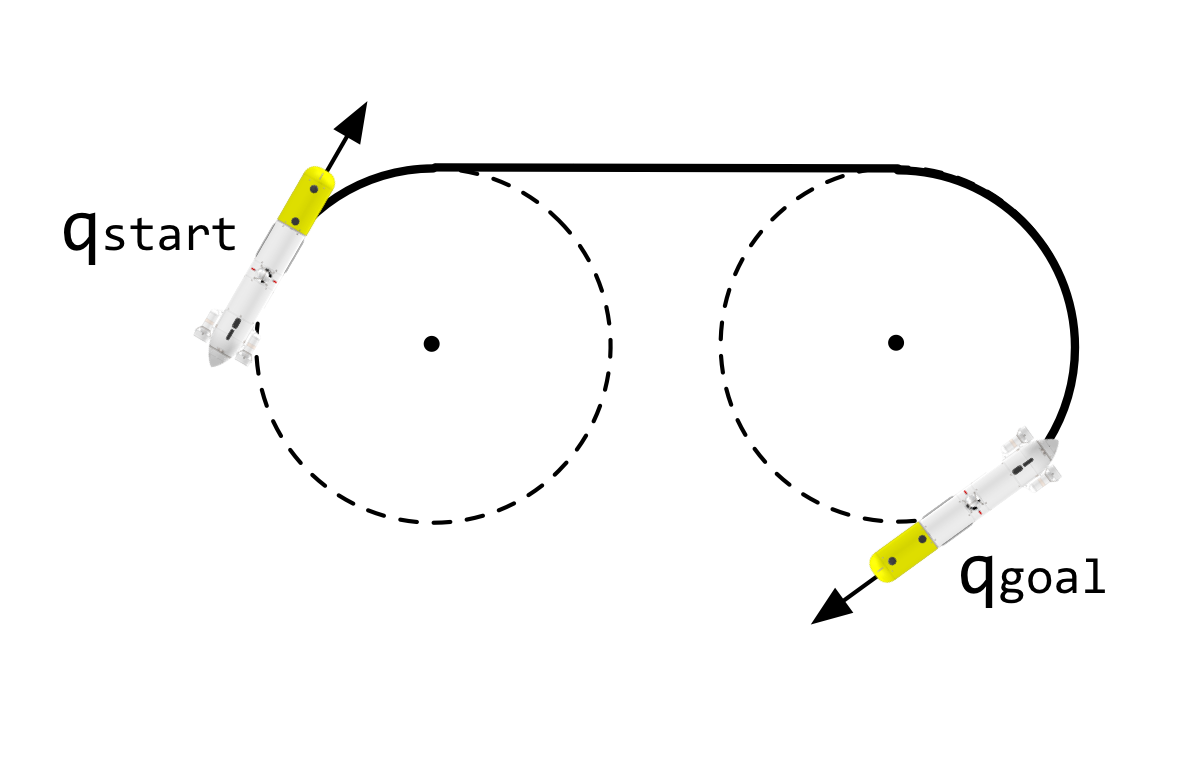
\includegraphics[width=.45\linewidth]{DubinsRSR}}\\%\quad
%     \subfloat[RLR]
%     {\label{fig:DubinsRLR}
%     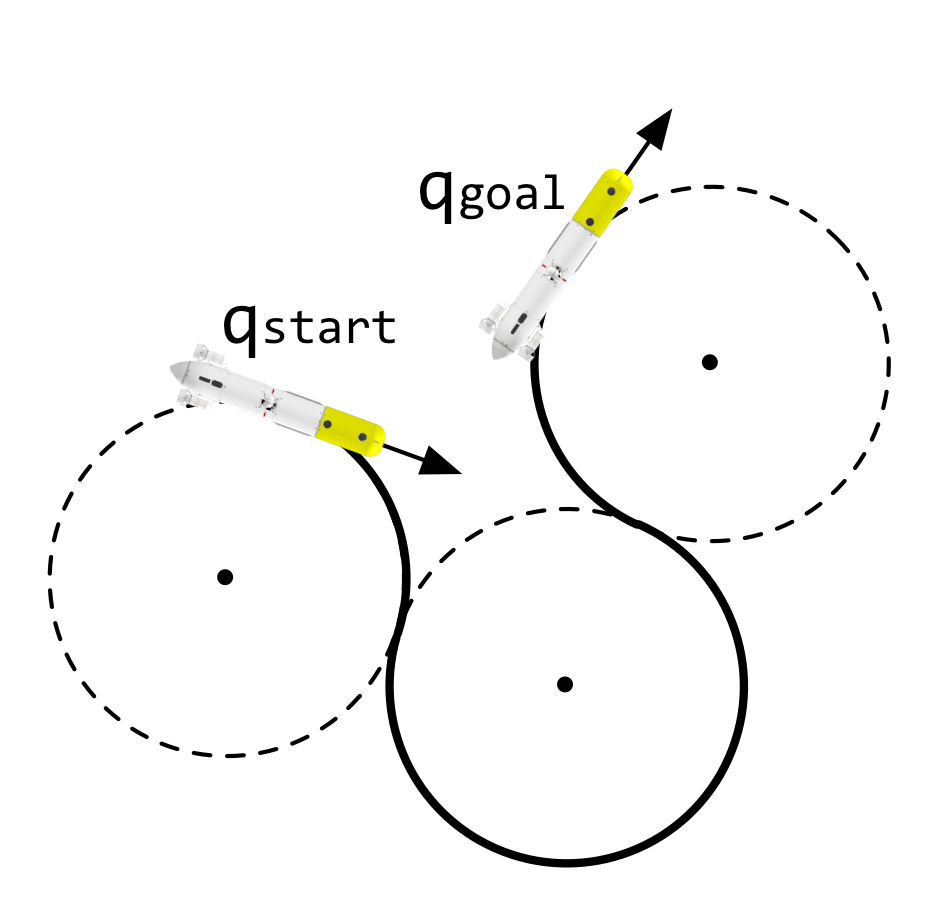
\includegraphics[width=.35\linewidth]{DubinsRLR}} \qquad
    \subfloat[LRL]
    {\label{fig:DubinsLRL}%
     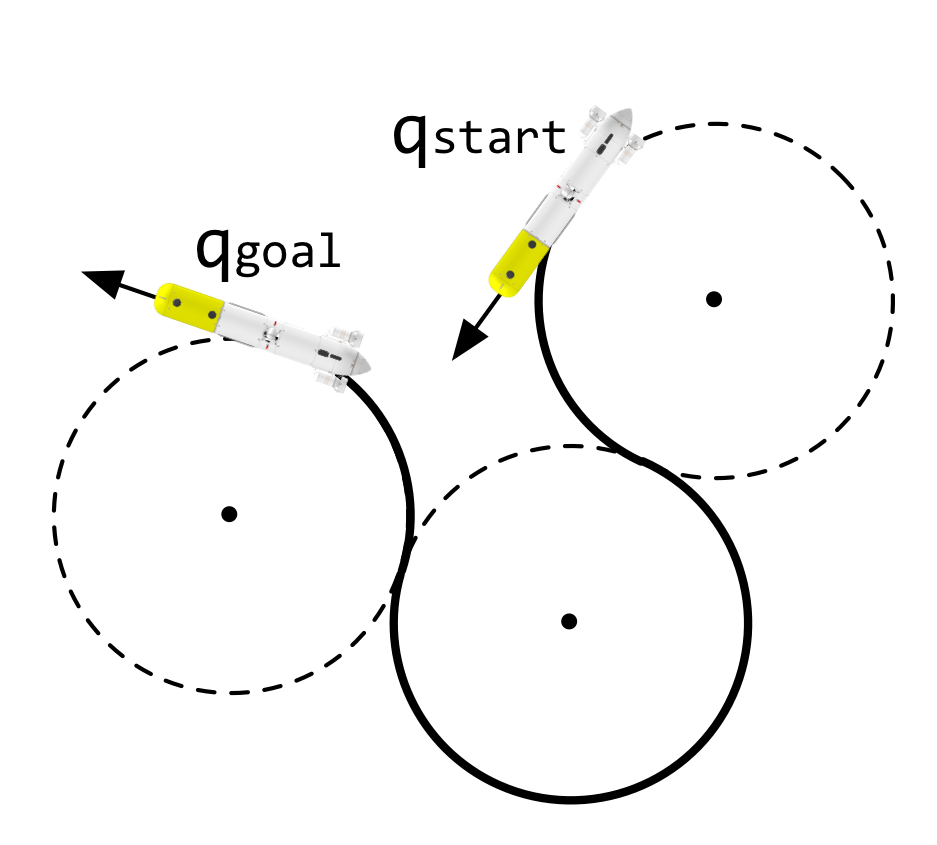
\includegraphics[width=.33\linewidth]{DubinsLRL}}
\caption[Examples of Dubins curves.]
{Examples of Dubins curves}
\label{fig:DubinsPathsExample}
\end{figure}

These constrained maneuvers are commonly used to describe feasible trajectories
for different ground, aerial, and underwater vehicles such as a torpedo-shaped
\ac{AUV}. For this latter case, Equation~\eqref{eq:KinEqAUV2D} describes an
\ac{AUV} that navigates at constant depth and with a constant surge speed $v$,
where the maximum turning rate $w_{max}$ establishes the minimum turning radius
$r_{min}$ for a Dubins vehicle. For both arcs and straight lines, this means
that for any given position $(x,y)$ over the path, its tangent angle corresponds
to the \ac{AUV} heading $(\psi)$, thus completing the state information
$q=[x,y,\psi]$.

This alternative formulation for the \ac{AUV} motion constraints can be used
with incremental search methods such as the \ac{RRT} variants. In such a case,
the control input $u_{near\_ to\_rand}$, required to evolve the system from
$q_{near}$ to $q_{rand}$ (Algorithm~\ref{alg:ExtendRRTDiffConstr},
line~\ref{alg_line:findInput}), can be replaced with Dubins curves (see
Fig.~\ref{fig:ExpansionRRTDubins}). Furthermore, it is important to note that
Dubins curves also work as a steering function, thus permitting to generate
near-optimal paths with an \ac{RRT*} algorithm.
Figure~\ref{fig:ReconnectionRRTstarDubins} depicts an example of how this
approach is used for reconnecting configurations near to $q_{new}$, thus
improving their associated cost. In this example the cost is assumed to be the path
length. Further details about Dubins curves are found in
%Appendix~\ref{appx:dubins_curves} and
references~\cite{Dubins1957},\cite{Shkel2001}.

\begin{figure}[htbp]
    \myfloatalign
    \subfloat[]
    {\label{fig:ExpansionRRTDubins-a}
    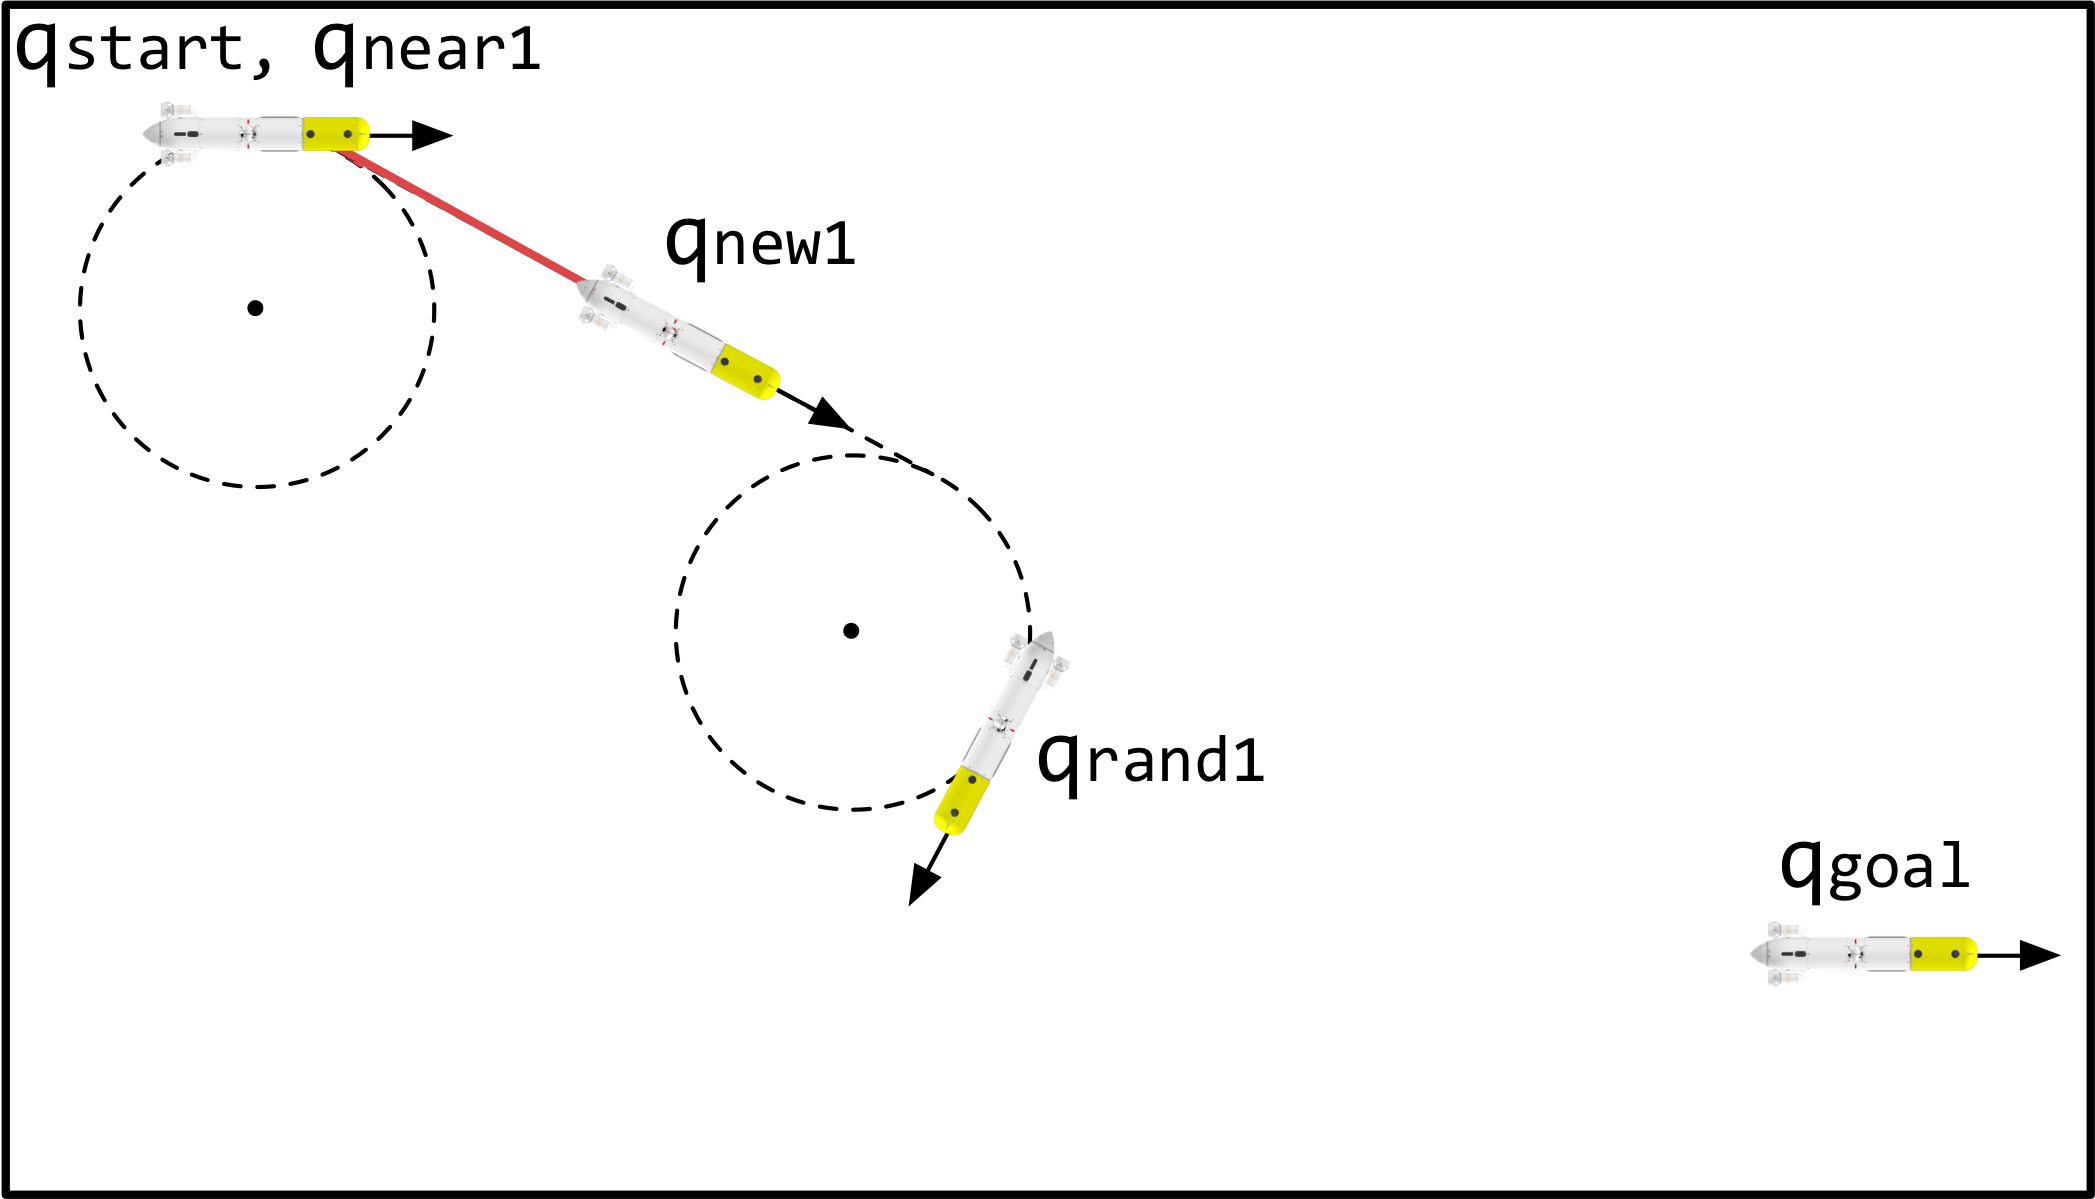
\includegraphics[width=.42\linewidth]{ExpansionRRTDubins-a}} \quad
    \subfloat[]
    {\label{fig:ExpansionRRTDubins-b}%
     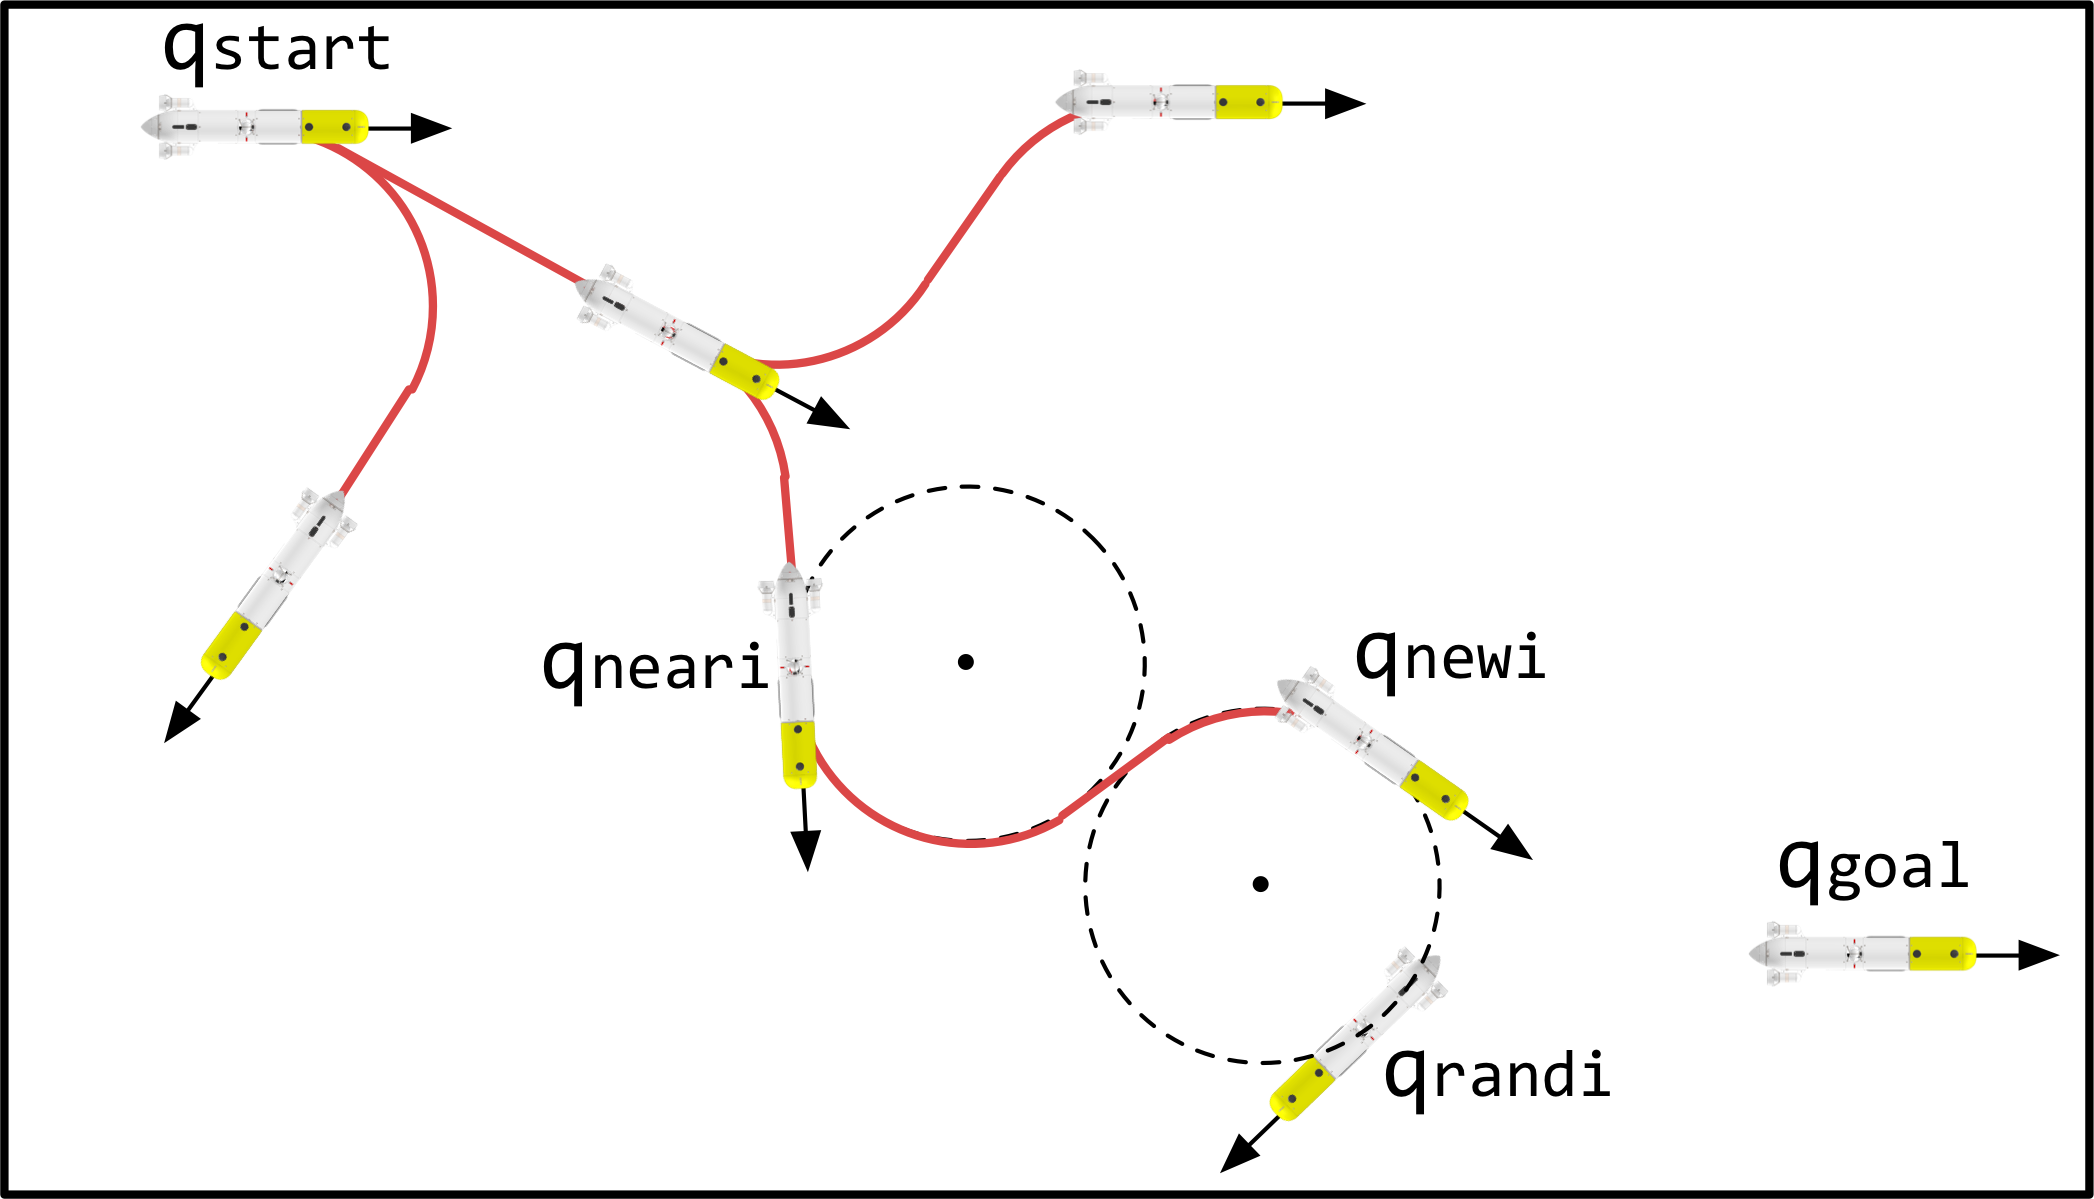
\includegraphics[width=.42\linewidth]{ExpansionRRTDubins-b}} \\
    \subfloat[]
    {\label{fig:ExpansionRRTDubinsComplete}
    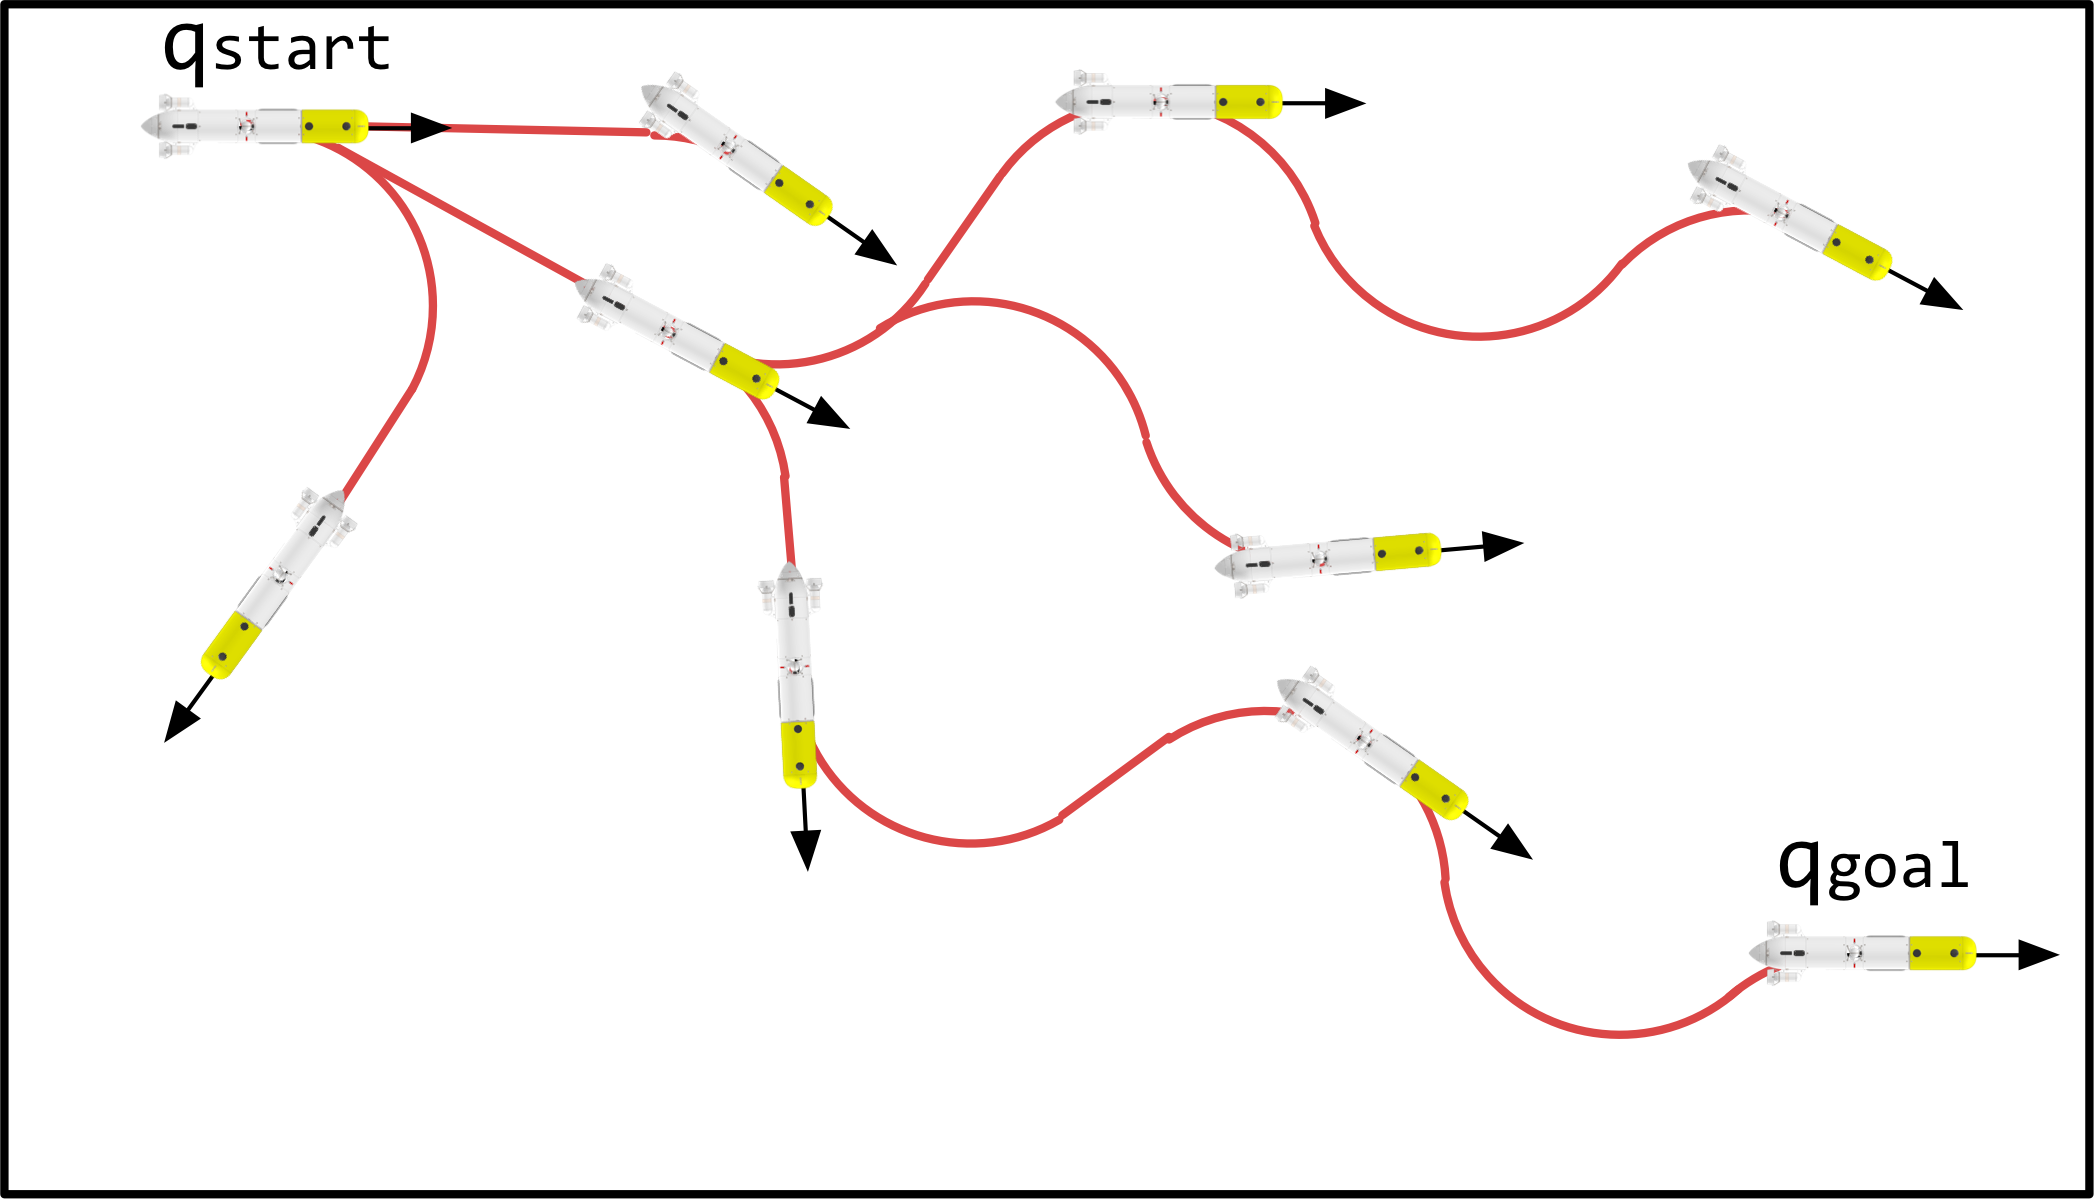
\includegraphics[width=.42\linewidth]{ExpansionRRTDubinsComplete}}
\caption[Start-to-goal query solution by expanding an RRT algorithm with Dubins
curves.] {Tree expansion of an \ac{RRT} algorithm that uses the Dubins curves.
\protect \subref{fig:RRTDiffConstrStep1} Given the start and goal states, a
first random sample is used to generate the first expansion of the tree
($q_{new}$).
\protect \subref{fig:ExpansionRRTDubins-b} The expansion $i^{th}$ of the tree.
\protect \subref{fig:RRTDiffConstrComplete} A feasible path has been found from
the start to the goal state.}
\label{fig:ExpansionRRTDubins}
\end{figure}

\begin{figure}[htbp]
    \myfloatalign
    \subfloat[]
    {\label{fig:ReconnectionRRTstarDubins-a}
    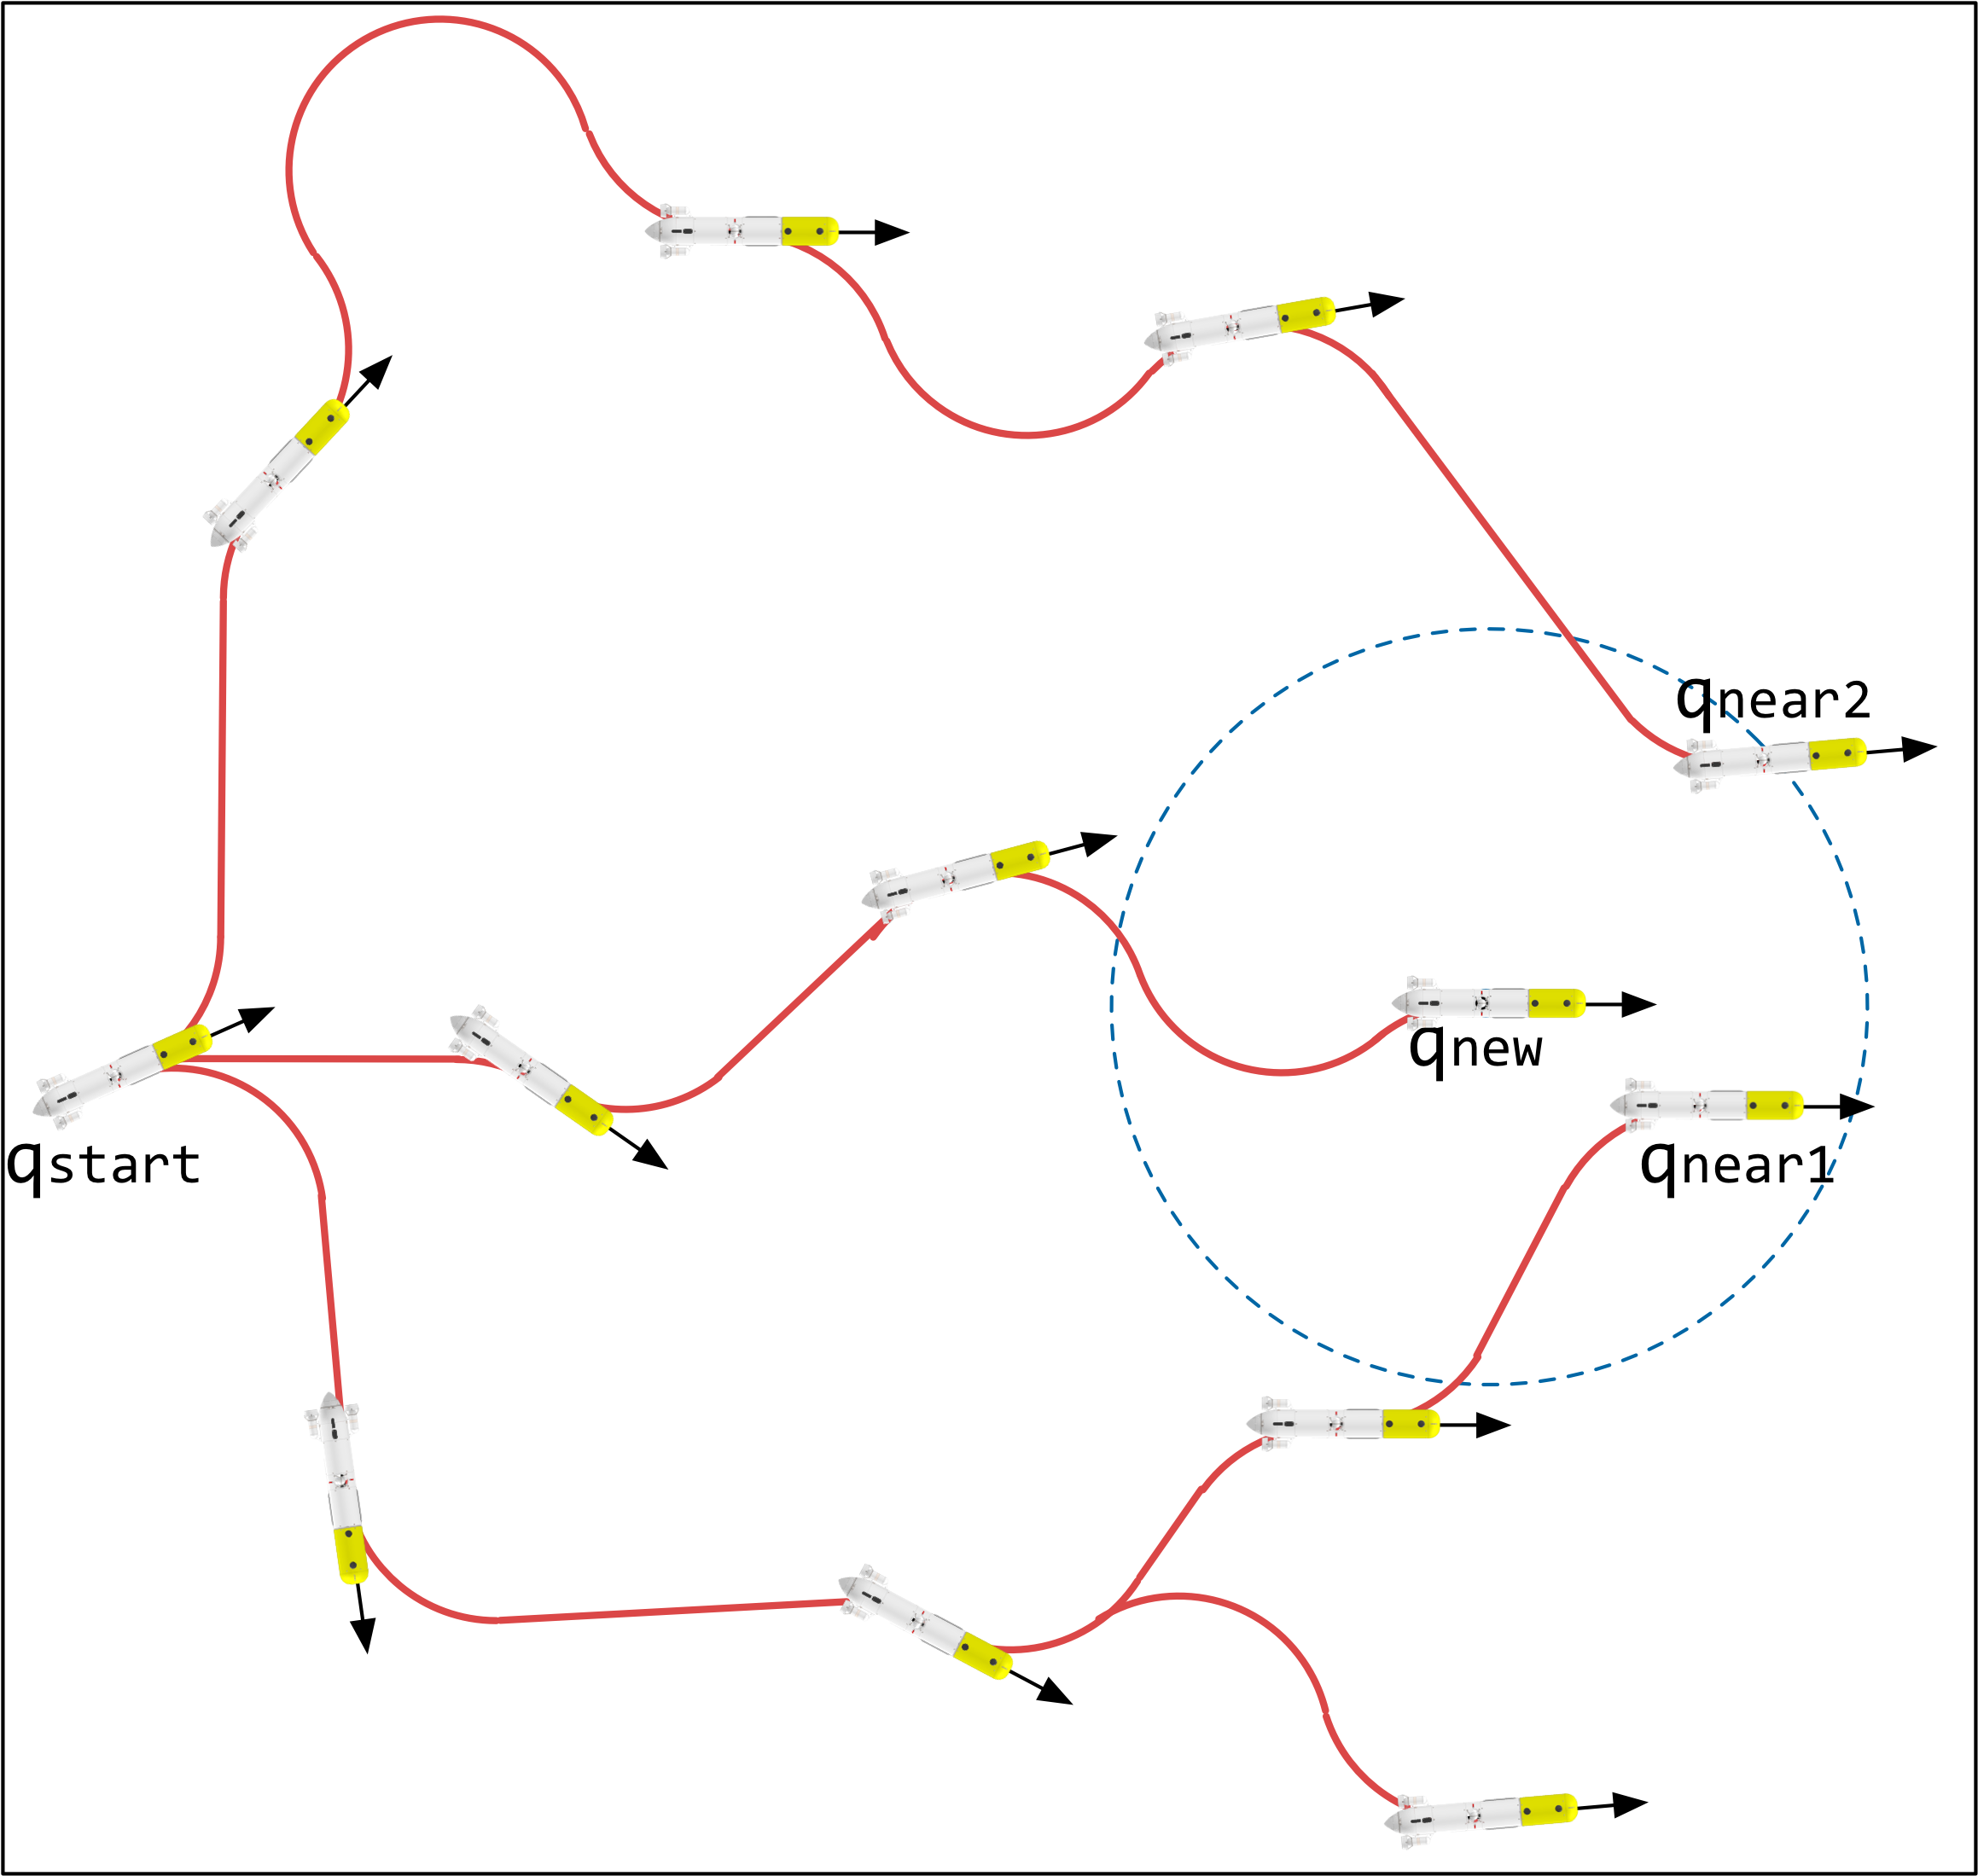
\includegraphics[width=.5\linewidth]{ReconnectionRRTstarDubins-a}} \quad
    \subfloat[]
    {\label{fig:ReconnectionRRTstarDubins-b}%
     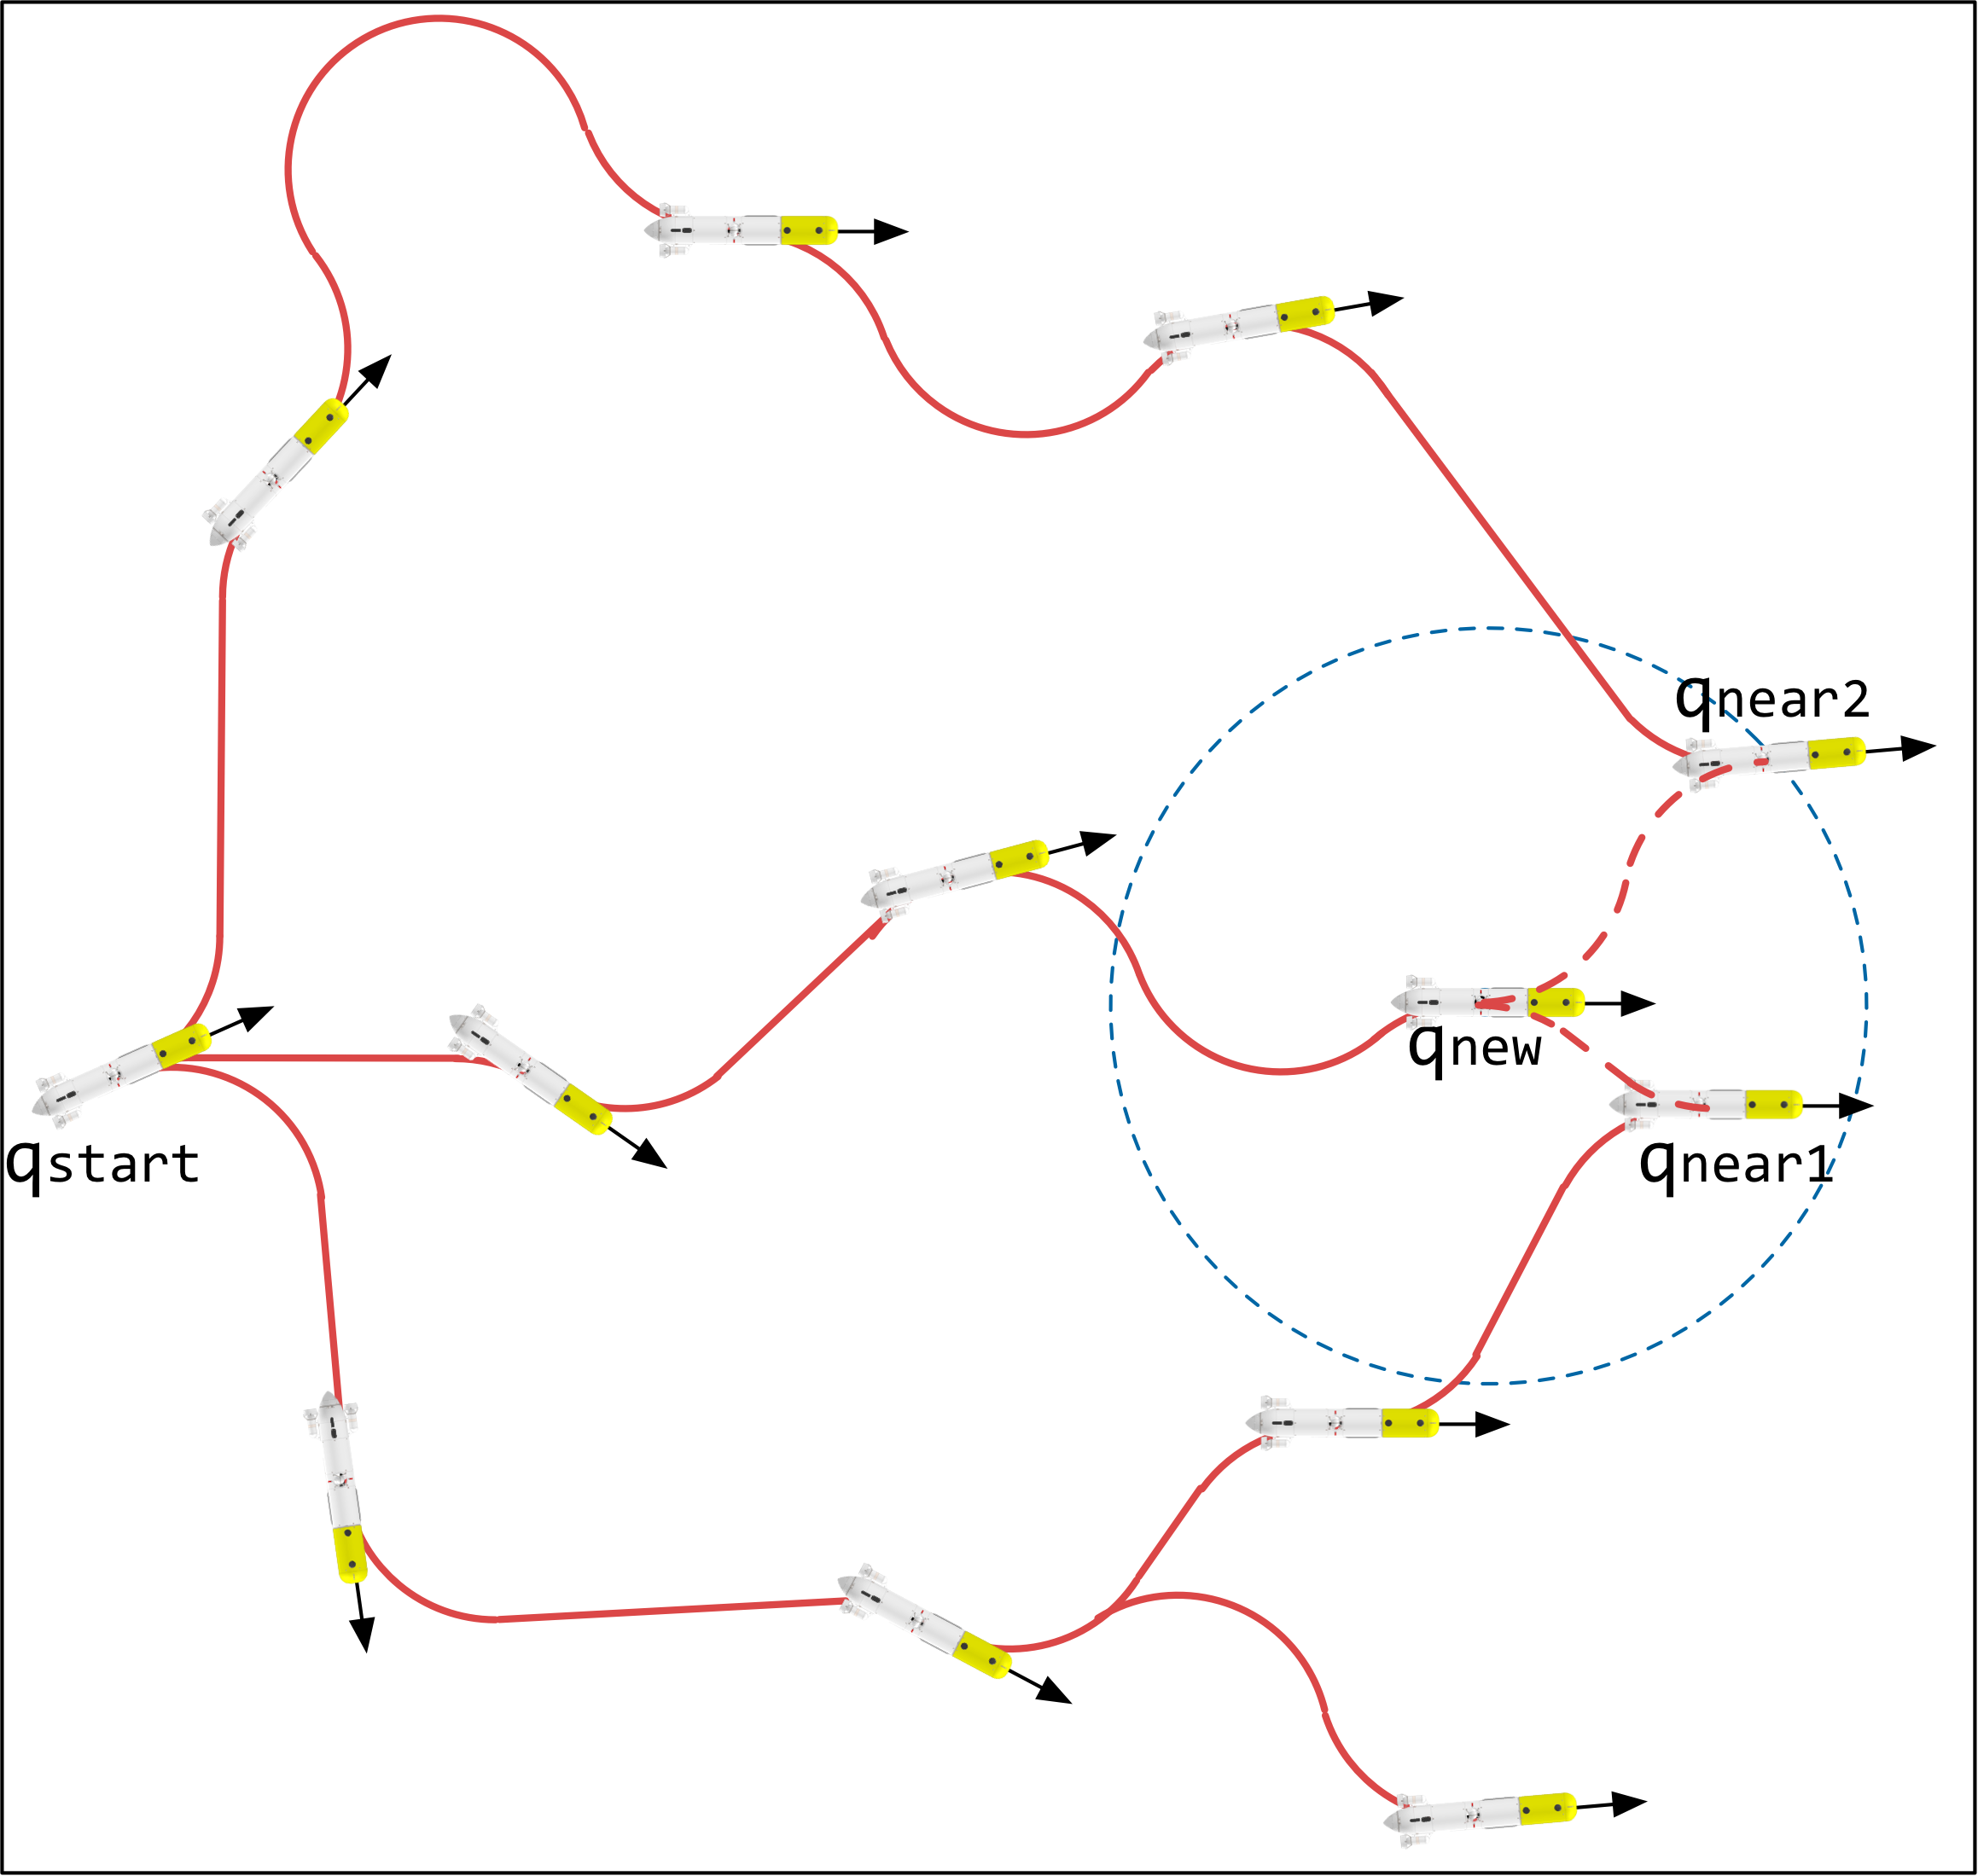
\includegraphics[width=.5\linewidth]{ReconnectionRRTstarDubins-b}} \quad
    \subfloat[]
    {\label{fig:ReconnectionRRTstarDubins-c}
    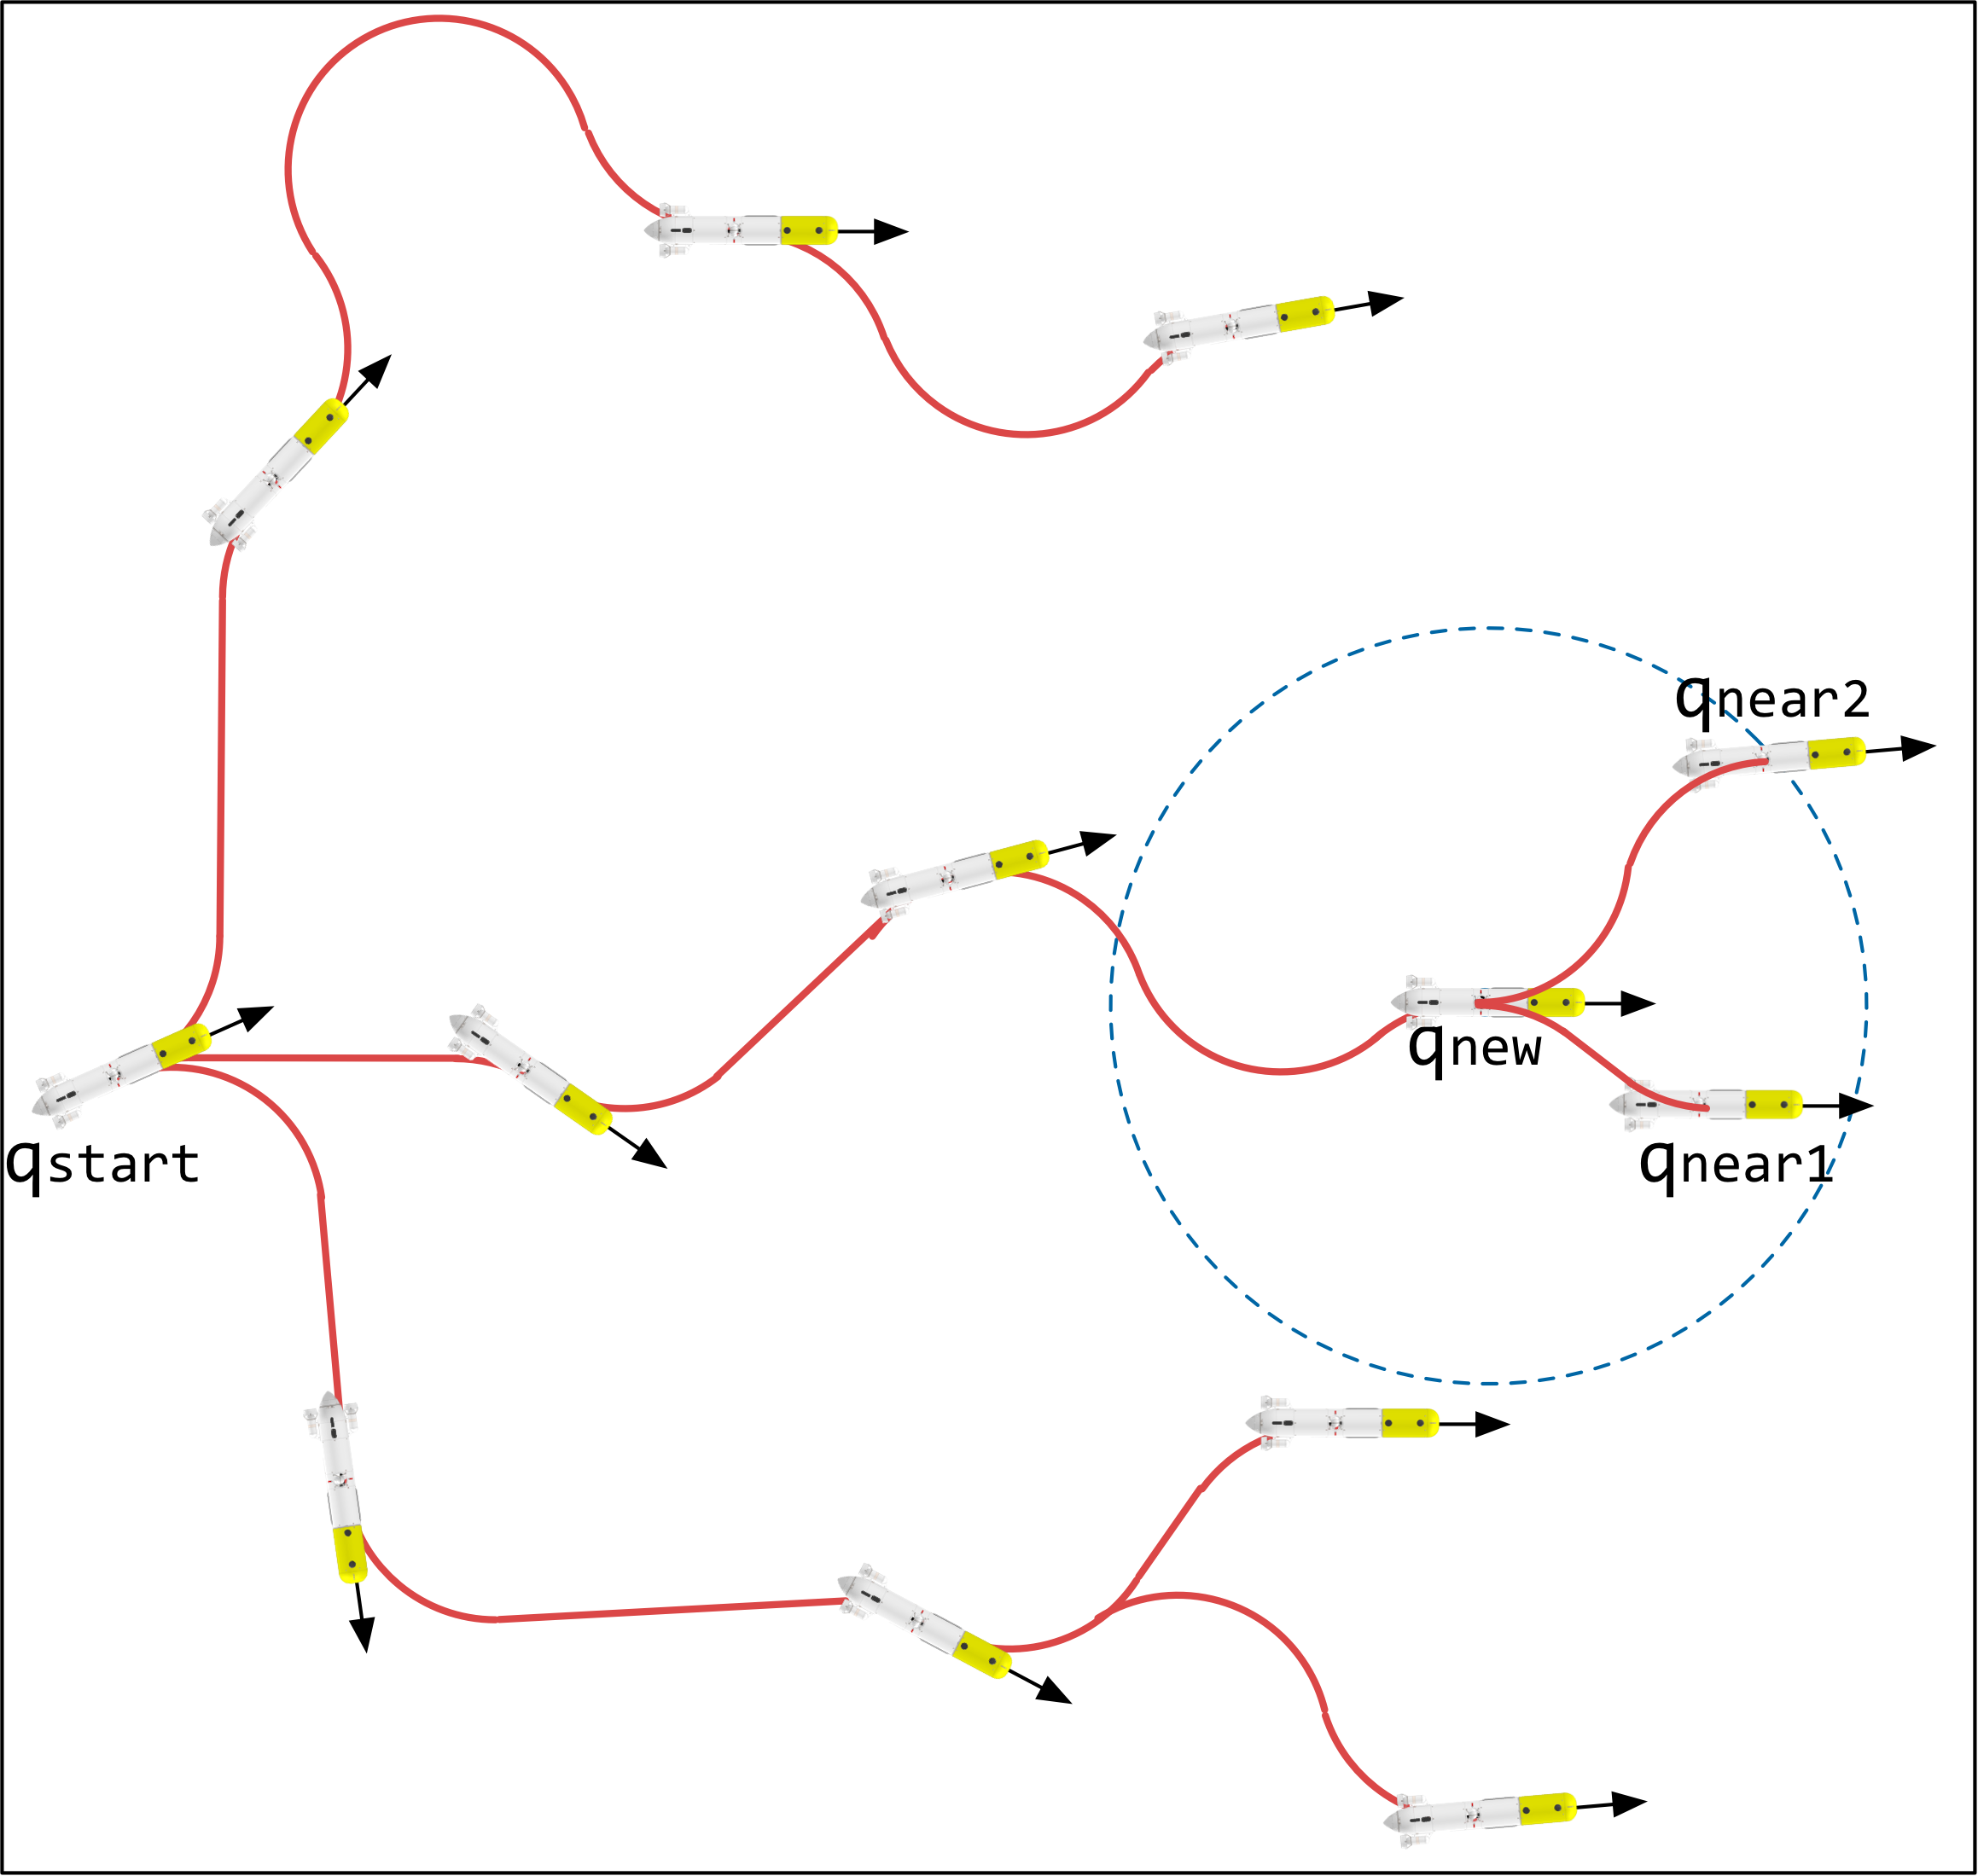
\includegraphics[width=.5\linewidth]{ReconnectionRRTstarDubins-c}}
\caption[RRT* algorithm reconnection using Dubins curves as steering function.]
{\ac{RRT*} algorithm reconnection using Dubins curves as steering function.
\protect \subref{fig:ReconnectionRRTstarDubins-a} Once a new configuration
$q_{new}$ has been obtained, 
\protect \subref{fig:ReconnectionRRTstarDubins-b} the \ac{RRT*} algorithm checks
if the nearest configurations to $q_{new}$ can be reconnected.
\protect \subref{fig:ReconnectionRRTstarDubins-c} If such a reconnection
decreases the cost associated with the nearest configurations, the new paths are
created while discarding the previous ones. This allows to progressively
improves the solution path.}
\label{fig:ReconnectionRRTstarDubins}
\end{figure}

Finally, in order to fully understand the aforementioned approaches, next
section presents solutions for different start-to-goal queries that have been
obtained using both geometric and motion constraints. Moreover, it also proves
the advantages of using Dubins curves instead of using a standard \ac{RRT}
algorithm by integrating Equation~\eqref{eq:KinEqAUV2D}.

\section{Results}

The main motivation behind the research presented throughout this thesis was the
need to plan more accurate motions that permit an \ac{AUV} to operate in
environments that are more complex. As explained in the Introduction, this
manuscript is organized in different chapters, each presenting the incremental
development of a motion planning framework that endows \acp{AUV} with such
capabilities. Therefore, the results presented and discussed in this section not
only tackled one of the proposed objectives, but largely established the
starting point for the rest of this research.

Having said that, the rest of this section seeks to prove the importance of
taking motion constraints into consideration when using non-holonomic \acp{AUV}.
To do so, simulation results present the Sparus~II \ac{AUV} conducting different
missions that were planned under both geometric and differential constraints. In
all cases, the vehicle navigated at a constant depth in a pre-explored
environment, \ie the obstacles and their locations were known.

\subsection{Conducting Missions under Geometric Constraints}

One simple alternative for planning paths for an \ac{AUV} that operates at
constant depth could be to approximate the vehicle to a point-like system, where
each configuration $q = [x,y] \in \mathbb{R}^2$. In such a case, an \ac{RRT*}
algorithm could generate (near) optimal paths if enough computing time is
provided. Figure~\ref{fig:PlannGeomConstr} depicts the solution path for a
start-to-goal query calculated for a point-like system using the \ac{RRT} and
the \ac{RRT*} algorithms, both under geometric constraints. However, in both
cases there are situations in which the path is so close to the obstacles that
it could lead to a collision if any real (non-point-like) vehicle would actually
try to follow the path. To prevent this, a simple solution is to increase either
the size of the obstacle or the size of the vehicle when checking for
collisions~\cite{Choset2005}.

\begin{figure}[htbp]
    \myfloatalign
    \subfloat[Solution obtained by an \ac{RRT}]
    {\label{fig:PlannGeomRRTScen2}%
     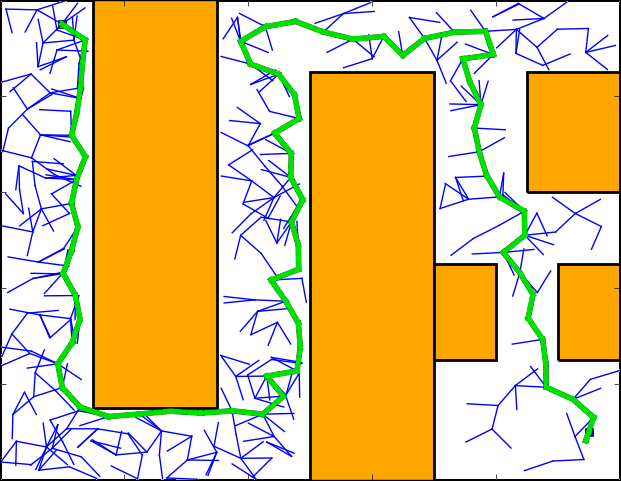
\includegraphics[width=.45\linewidth]{PlannGeomRRTScen2}}\quad
    \subfloat[Solution obtained by an \ac{RRT*}]
    {\label{fig:PlannGeomRRTstarScen2}%
     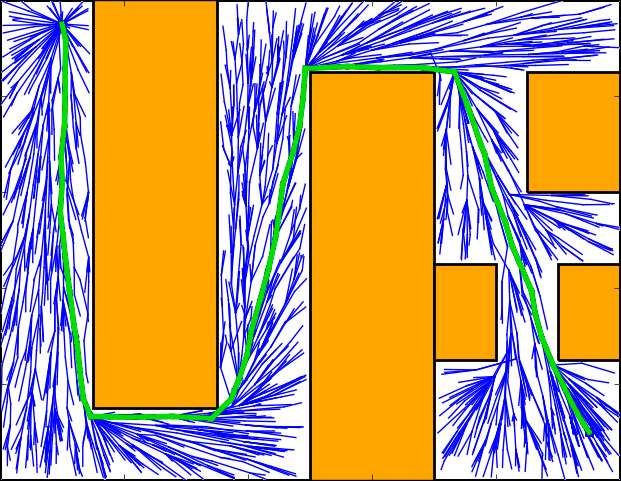
\includegraphics[width=.45\linewidth]{PlannGeomRRTstarScen2}}
\caption[Comparison between start-to-goal query solutions obtained by an RRT and
an RRT* algorithms over a 2D workspace.]
{Start-to-goal query solution for a point-like system using both \protect
\subref{fig:PlannGeomRRTScen2} the \ac{RRT} and \protect
\subref{fig:PlannGeomRRTstarScen2} the \ac{RRT*} algorithms. The simulated
scenario is composed of a series of polygonal obstacles presented in orange, the
safe or collision-free space in red, the tree branches in blue, and the solution
path in green.}
\label{fig:PlannGeomConstr}
\end{figure}

Nonetheless, even if the shape checked for collision is enlarged, it does not
guarantee that a vehicle can accurately follow the path.
Figure~\ref{fig:PlannGeomRRTstarQueries} depicts this situation in a simulated
scenario composed of two obstacles that create a narrow passage. In this
scenario, two different start-to-goal queries were defined in such a way that
required the solution path to be amidst the obstacles. Such paths were
calculated by an \ac{RRT*} algorithm under geometric constraints. In both cases,
a simulated Sparus~II \ac{AUV} attempted to follow the path, however new risky
situations appeared when conducting turning maneuvers. This occurred because the
planner, over $\mathcal{C}=\mathbb{R}^2$, does not consider the vehicle motion
limits (constraints) but, instead, it assumes the capability of instantaneously
changing the vehicle direction of motion. It is also important to highlight that
despite the fact that the executions of the missions were collision-free, the
\ac{AUV} surge speed and turning rate could have been established in a way that
would have made the vehicle collide with the obstacles.

\begin{figure}[htbp]
    \myfloatalign
%     \subfloat[\ldots.]
%     {\label{fig:PlannGeomRRTstarQ1Sol}
%     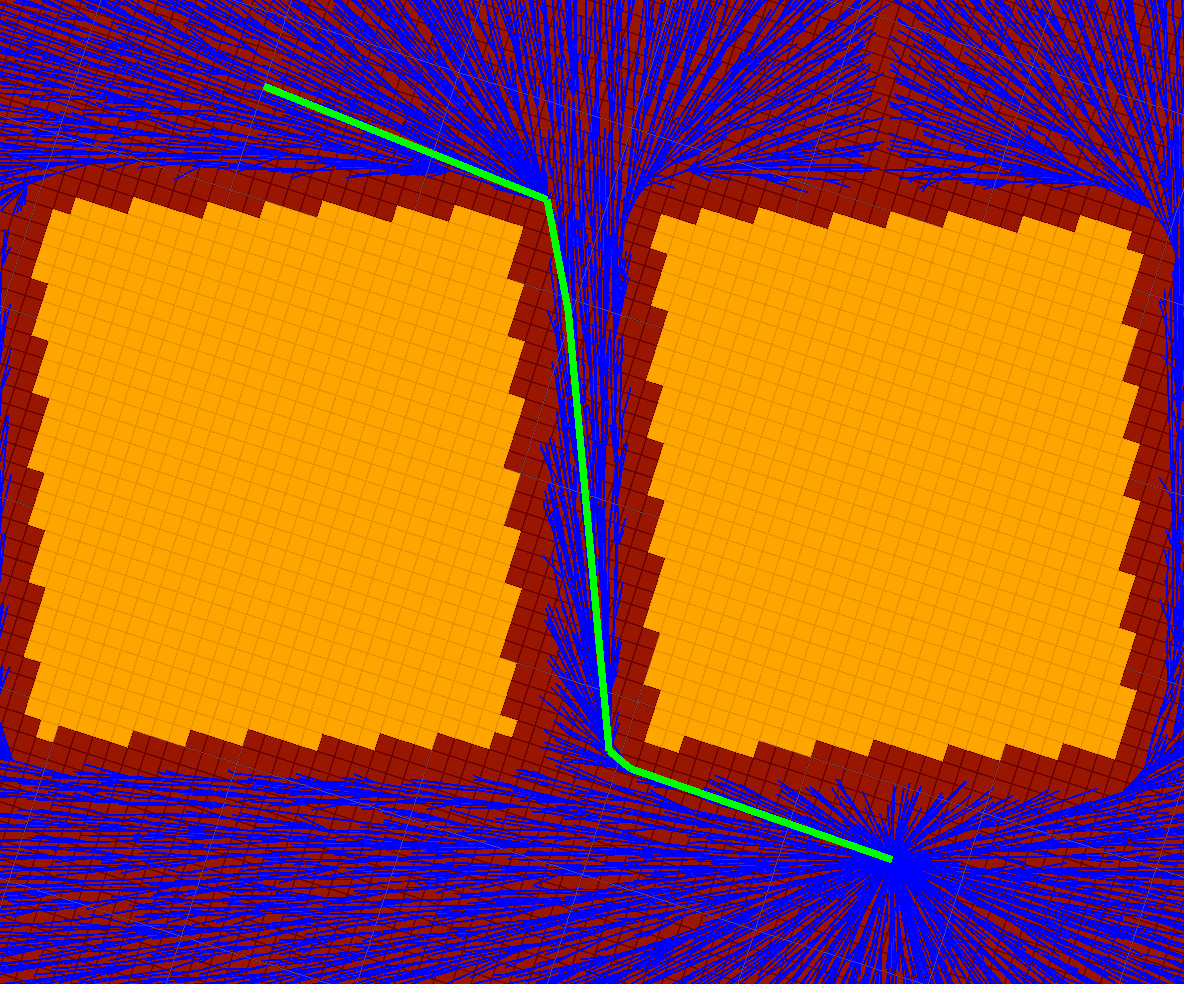
\includegraphics[width=.45\linewidth]{PlannGeomRRTstarQ1Sol}} \quad
%     \subfloat[\ldots]
%     {\label{fig:PlannGeomRRTstarQ2Sol}%
%      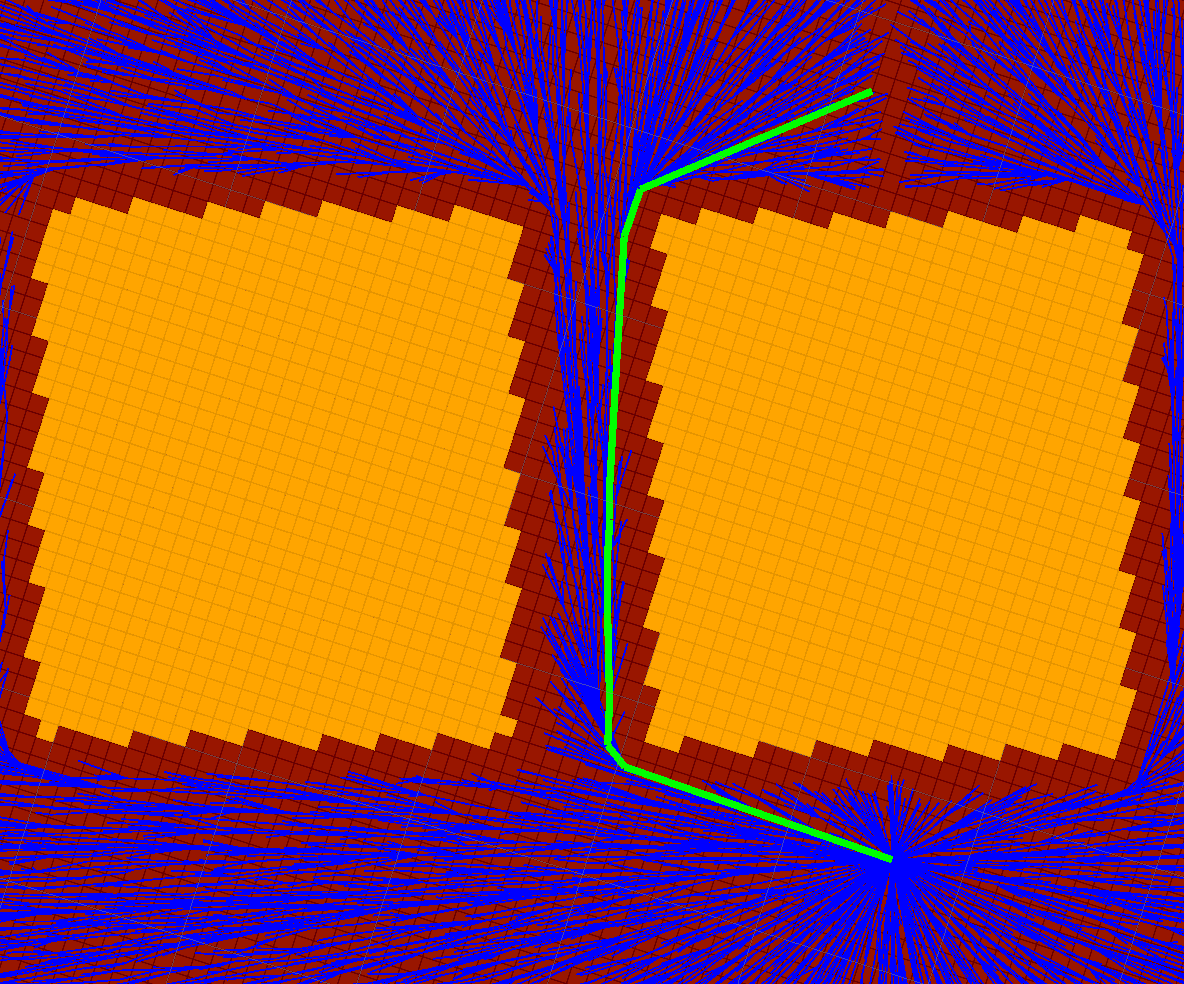
\includegraphics[width=.45\linewidth]{PlannGeomRRTstarQ2Sol}}\\
    \subfloat[Query 1]
    {\label{fig:PlannGeomRRTstarQ1Miss}
    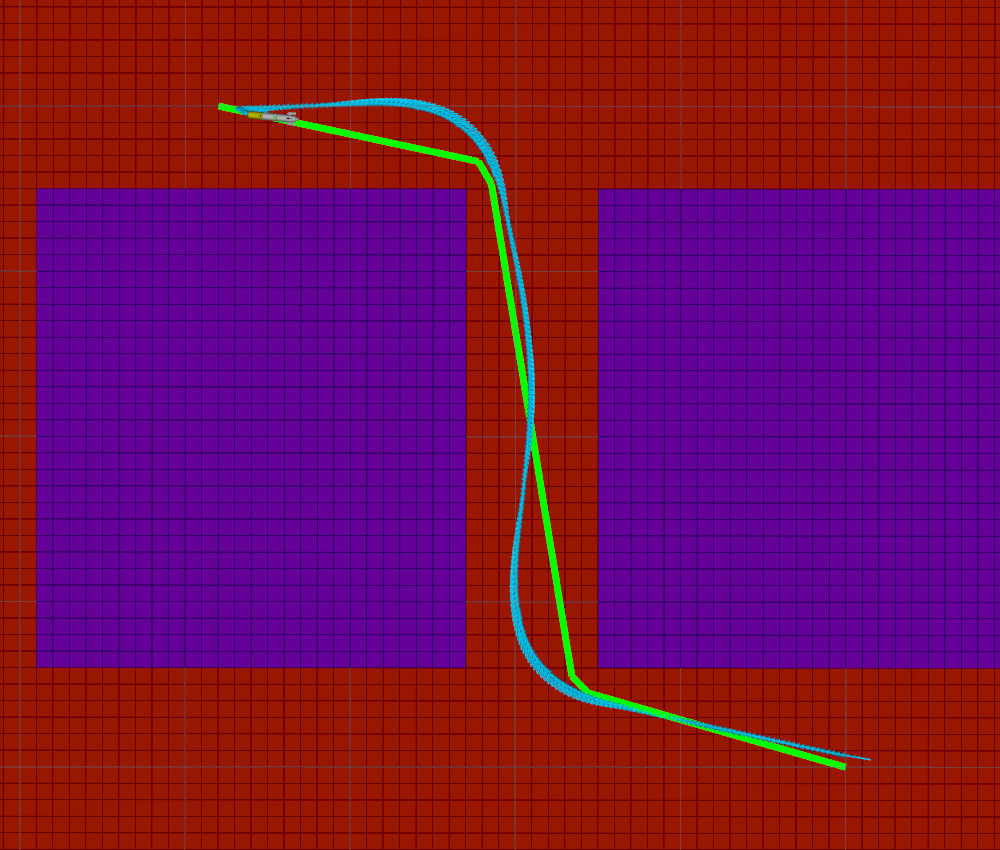
\includegraphics[width=.45\linewidth]{PlannGeomRRTstarQ1Miss}} \quad
    \subfloat[Query 2]
    {\label{fig:PlannGeomRRTstarQ2Miss}%
     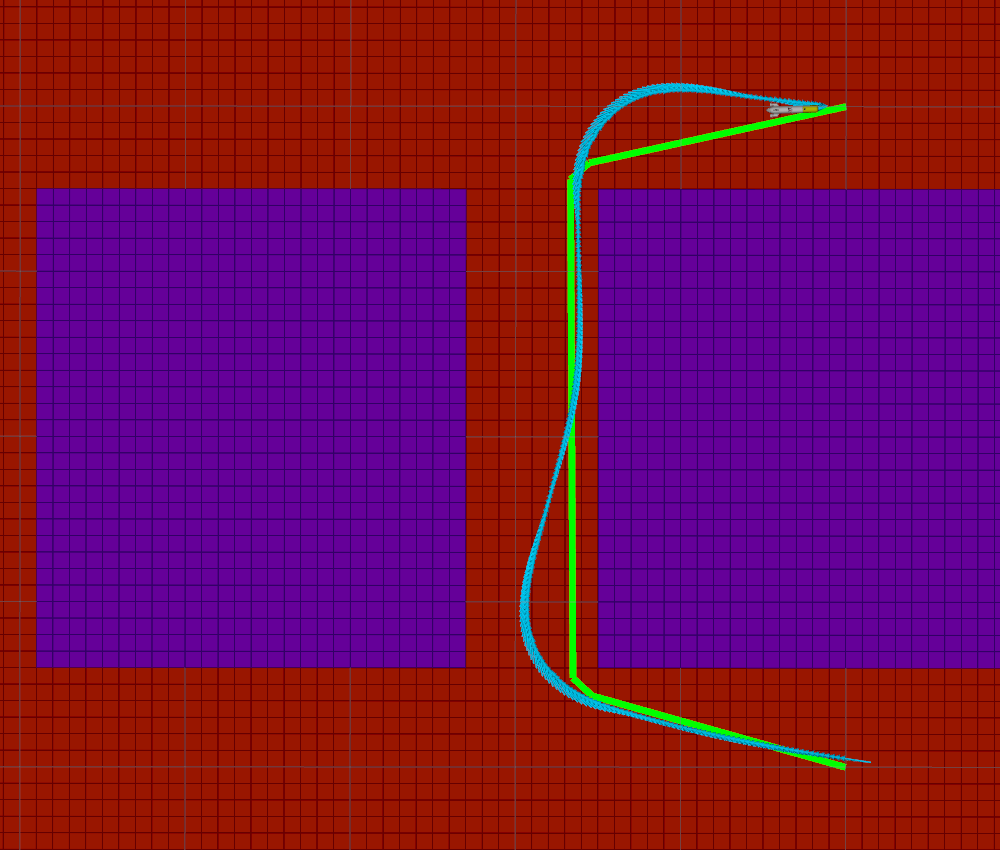
\includegraphics[width=.45\linewidth]{PlannGeomRRTstarQ2Miss}}
\caption[Simulation of the Sparus~II AUV attempting to follow a solution path
calculated by an RRT* under geometric constraints.]
{Simulated environment composed of two obstacles that create a narrow passage.
Two different start-to-goal query solutions that were calculated by an \ac{RRT*}
algorithm under geometric constraints are shown in green. A simulated Sparus~II
\ac{AUV} attempted to follow the paths, however the resulting vehicle trajectory
(in light blue) differs from the one calculated, thus leading to risky
situations when conducting turning maneuvers.}
\label{fig:PlannGeomRRTstarQueries}
\end{figure}

\subsection{Conducting Missions under Motion Constraints}

As explained along previous sections, a more appropriate formulation to limit
unexpected vehicle trajectories when following a path is to use a planner that
incorporates motion constraints. In such a case, the planner must not only
specify the position and orientation, but also use the vehicle equation of
motion.
% Figure~\ref{fig:PlannGeomDiffConstr}, for instance, depicts a situation in which
% using this formulation results decisive for planning doable motions for a
% unicycle-like vehicle.
% 
% \begin{figure}[htbp]
%     \myfloatalign
%     \subfloat[Solution obtained by an \ac{RRT*}.]
%     {\label{fig:PlannGeomRRTstarScen3}
%     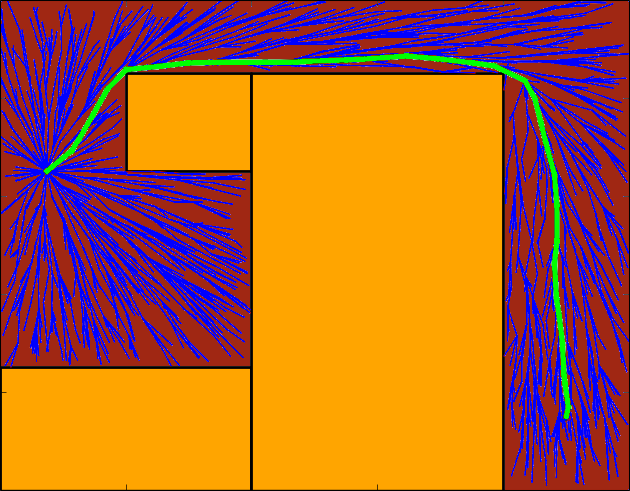
\includegraphics[width=.45\linewidth]{PlannGeomRRTstarScen3}} \quad
%     \subfloat[Solution obtained by an \ac{RRT}.]
%     {\label{fig:PlannConstRRTScen3}%
%      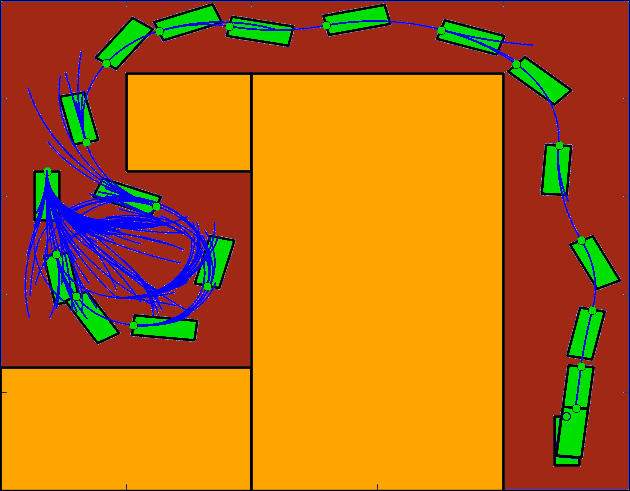
\includegraphics[width=.45\linewidth]{PlannConstRRTScen3}}
%     \caption{Start-to-goal query solutions that were obtained by \protect
%     \subref{fig:PlannGeomRRTScen2} an \ac{RRT*} under geometric constraints for
%     a point-like system, and \protect \subref{fig:PlannConstRRTScen3} an
%     \ac{RRT} under motion constraints that uses the unicycle equation of
%     motion.}
%     \label{fig:PlannGeomDiffConstr}
% \end{figure}
For the particular case of a torpedo-shaped \ac{AUV}, this chapter explained two
alternatives to incorporate Eq.~\eqref{eq:KinEqAUV2D} into the motion planner.
In order to compare the approaches, both were used to solve the same
start-to-goal queries presented in Fig.~\ref{fig:PlannGeomRRTstarQueries}. For
the first alternative, Figures~\ref{fig:PlannKinodRRTQ1Miss}
and~\ref{fig:PlannKinodRRTQ2Miss} depict a simulated Sparus~II \ac{AUV}
following solution paths that were calculated by an \ac{RRT} algorithm that
mathematically integrates Eq.~\eqref{eq:KinEqAUV2D}. In this case, the \ac{RRT}
algorithm does not provide any guarantee for optimality.

\begin{figure}[htbp]
    \myfloatalign
    \subfloat[RRT: Query 1]
    {\label{fig:PlannKinodRRTQ1Miss}
    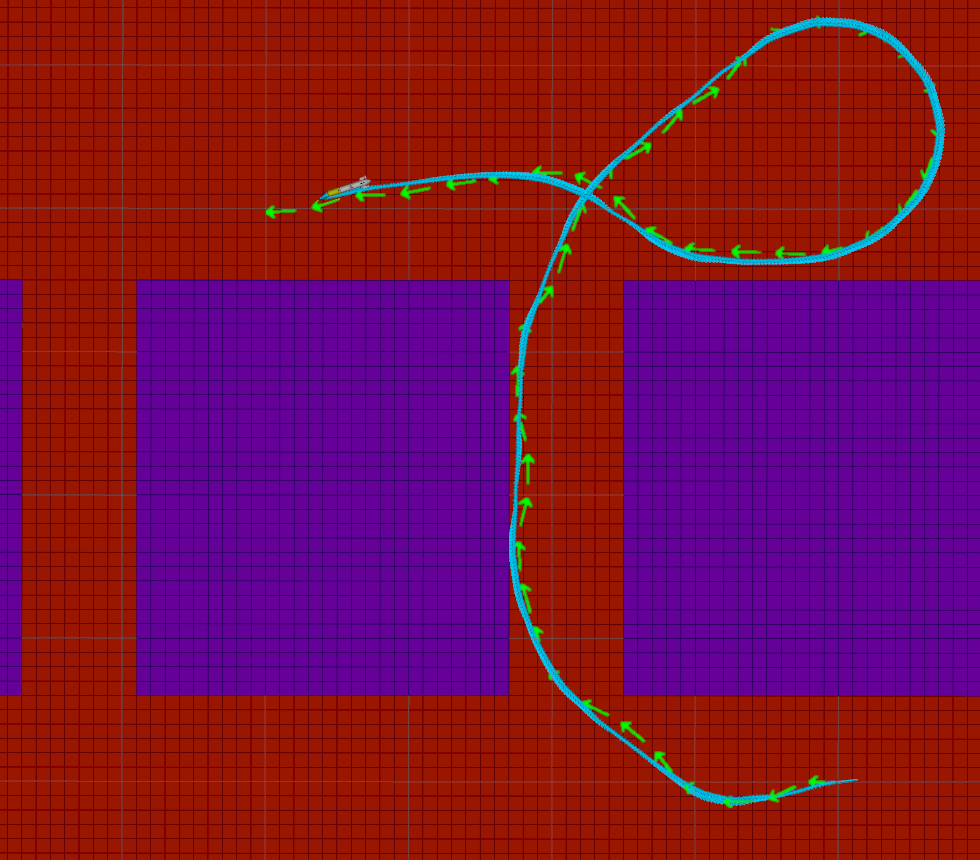
\includegraphics[width=.45\linewidth]{PlannKinodRRTQ1Miss}} \quad
    \subfloat[RRT: Query 2]
    {\label{fig:PlannKinodRRTQ2Miss}%
     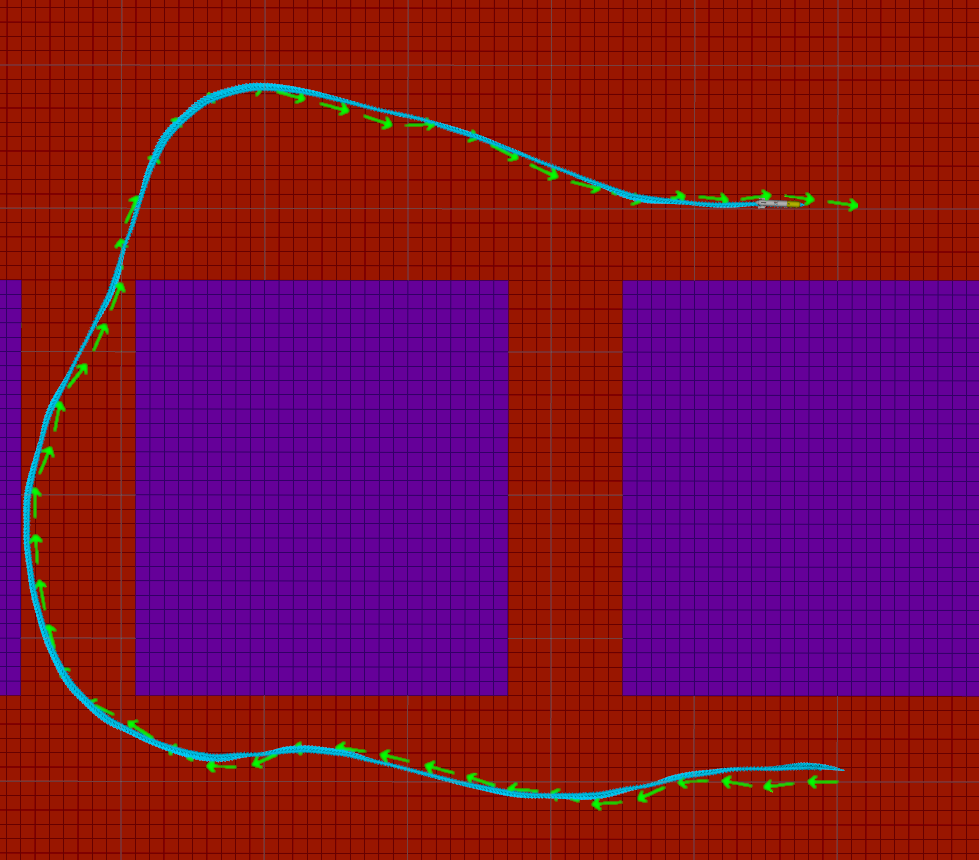
\includegraphics[width=.45\linewidth]{PlannKinodRRTQ2Miss}}\\
   \subfloat[RRT* with Dubins: Query 1]
    {\label{fig:PlannDubinsRRTstarQ1Miss}
    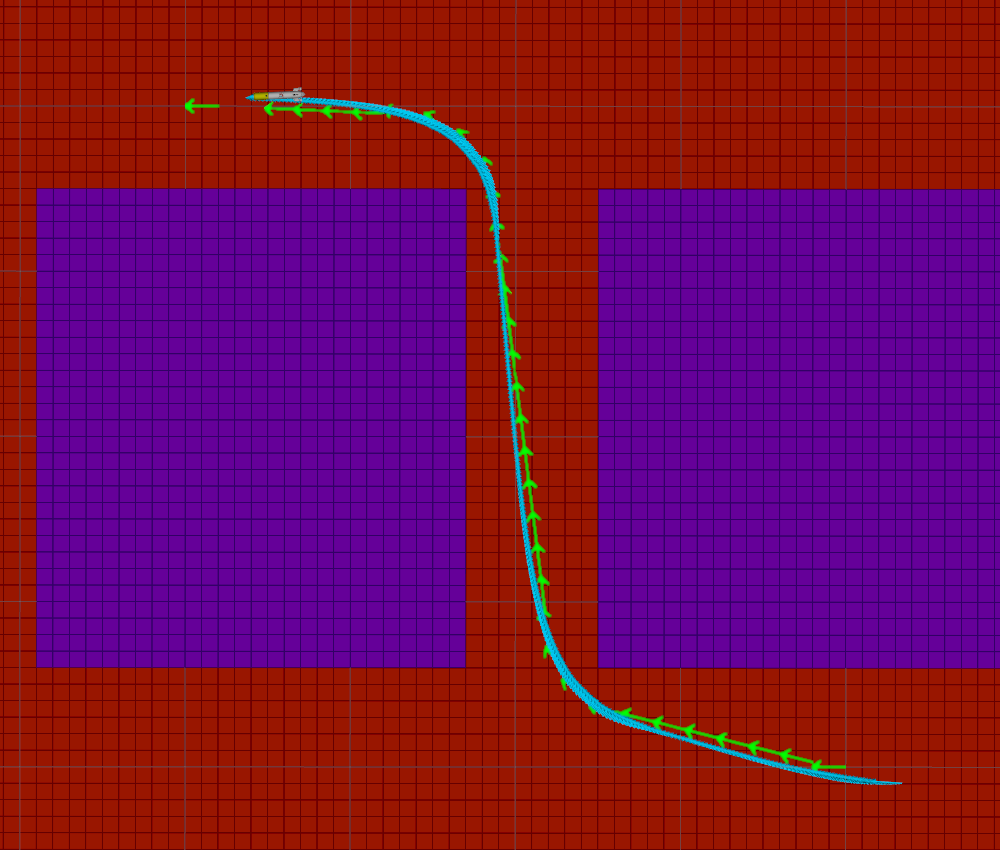
\includegraphics[width=.45\linewidth]{PlannDubinsRRTstarQ1Miss}} \quad
    \subfloat[RRT* with Dubins: Query 2]
    {\label{fig:PlannDubinsRRTstarQ2Miss}%
     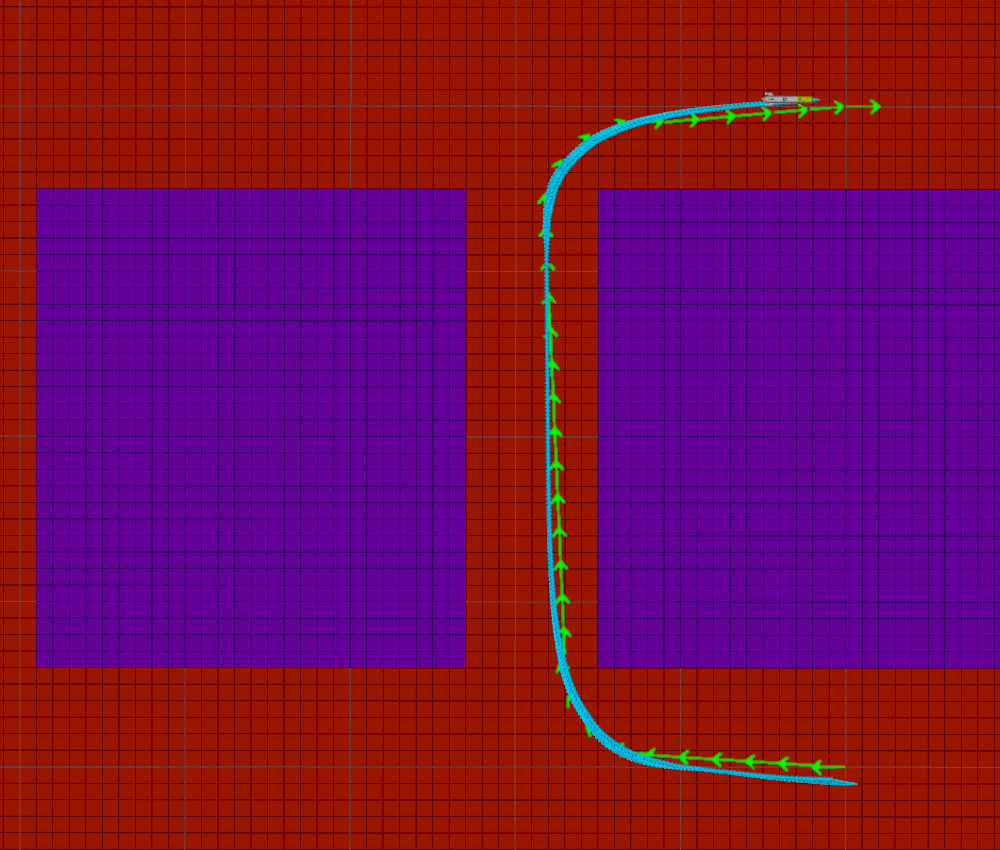
\includegraphics[width=.45\linewidth]{PlannDubinsRRTstarQ2Miss}}
\caption[Simulation of the Sparus~II AUV attempting to follow a solution path
calculated by an RRT and RRT* under motion constraints.]
{Simulated environment composed of obstacles that create narrow
passages. Sparus~II \ac{AUV} follows the calculated paths. 
\protect \subref{fig:PlannKinodRRTQ1Miss}, \protect
\subref{fig:PlannKinodRRTQ2Miss} Two different start-to-goal query solutions
that were calculated by an \ac{RRT} algorithm under motion constraints are shown
in green. In this case, the \ac{RRT} algorithm does not provide any guarantee
for optimality.
\protect \subref{fig:PlannDubinsRRTstarQ1Miss}, \protect
\subref{fig:PlannDubinsRRTstarQ2Miss} The same start-to-goal queries were
solved by an \ac{RRT*} algorithm with Dubins curves as steering function.
Solutions are shown in green.}
\label{fig:PlannKinodRRTQueries}
\end{figure}

% \begin{figure}[htbp]
%     \myfloatalign
% %     \subfloat[\ldots.]
% %     {\label{fig:PlannKinodRRTQ1Sol}
% %     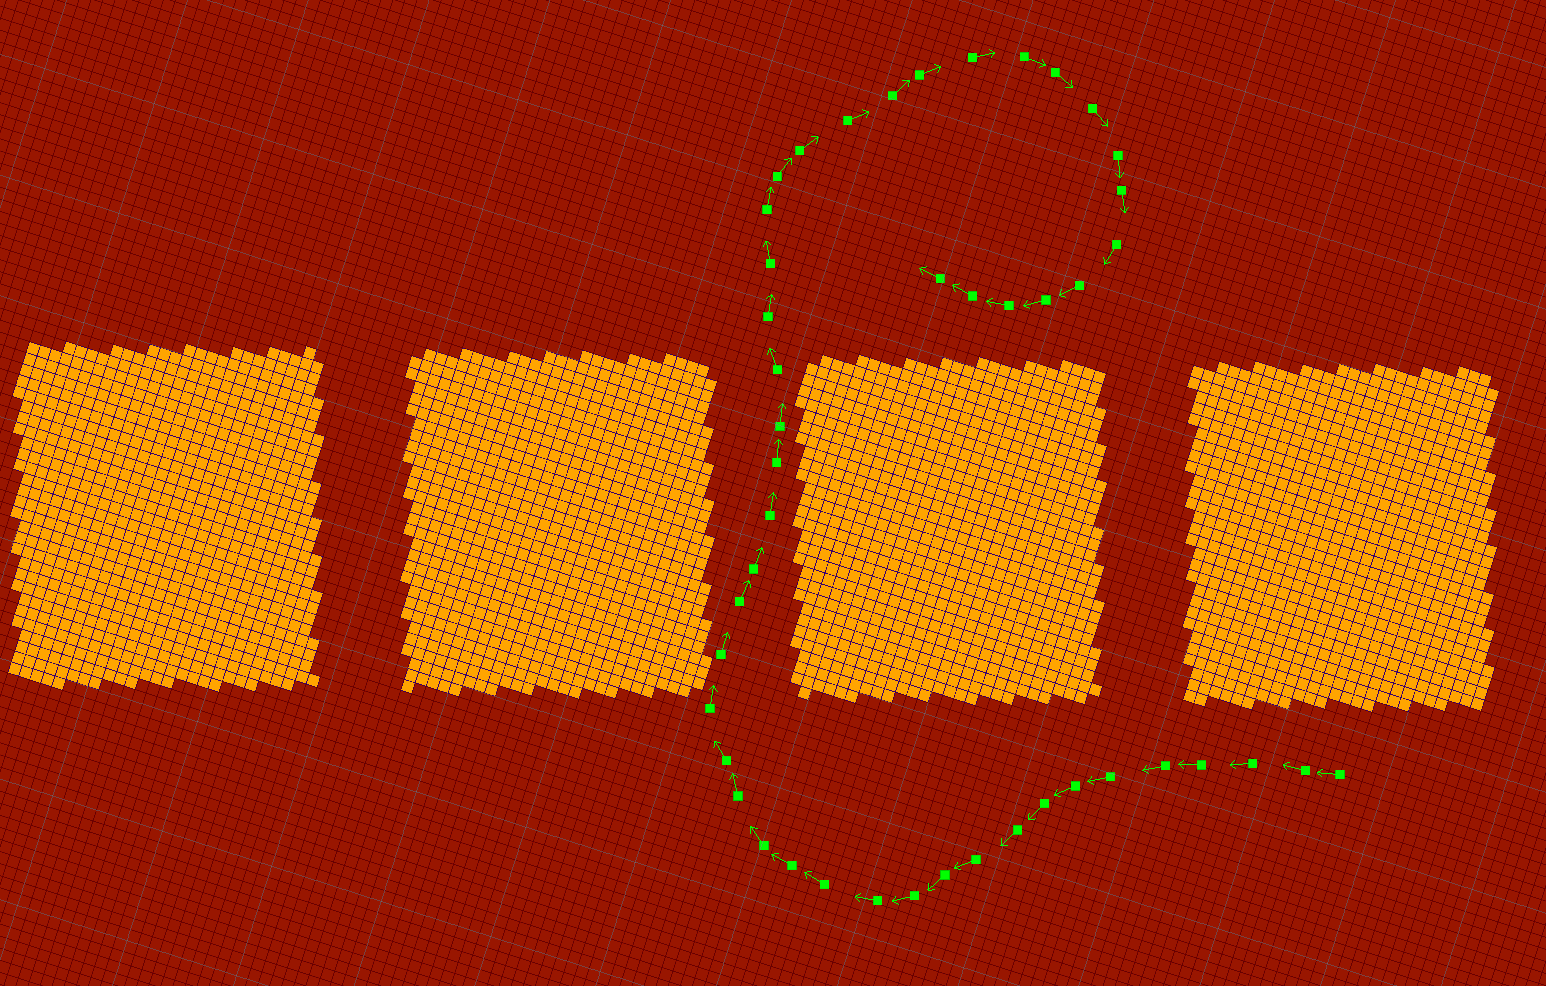
\includegraphics[width=.45\linewidth]{PlannKinodRRTQ1Sol}} \quad
% %     \subfloat[\ldots]
% %     {\label{fig:PlannKinodRRTQ2Sol}%
% %      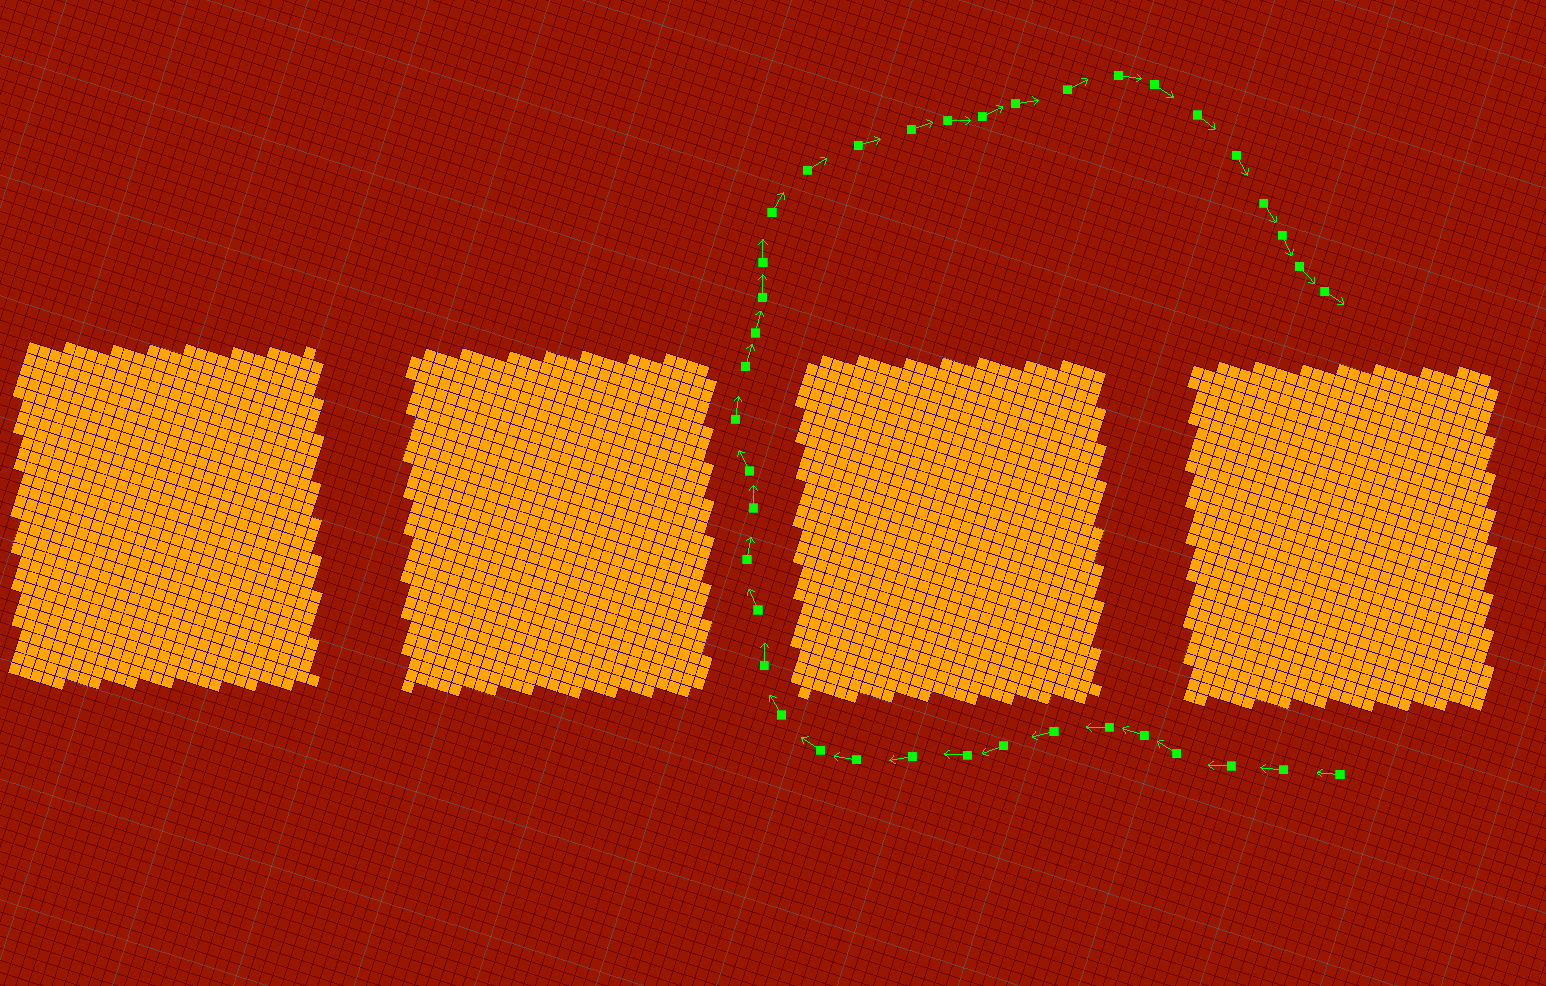
\includegraphics[width=.45\linewidth]{PlannKinodRRTQ2Sol}}\\
%     \subfloat[Query 1]
%     {\label{fig:PlannKinodRRTQ1Miss}
%     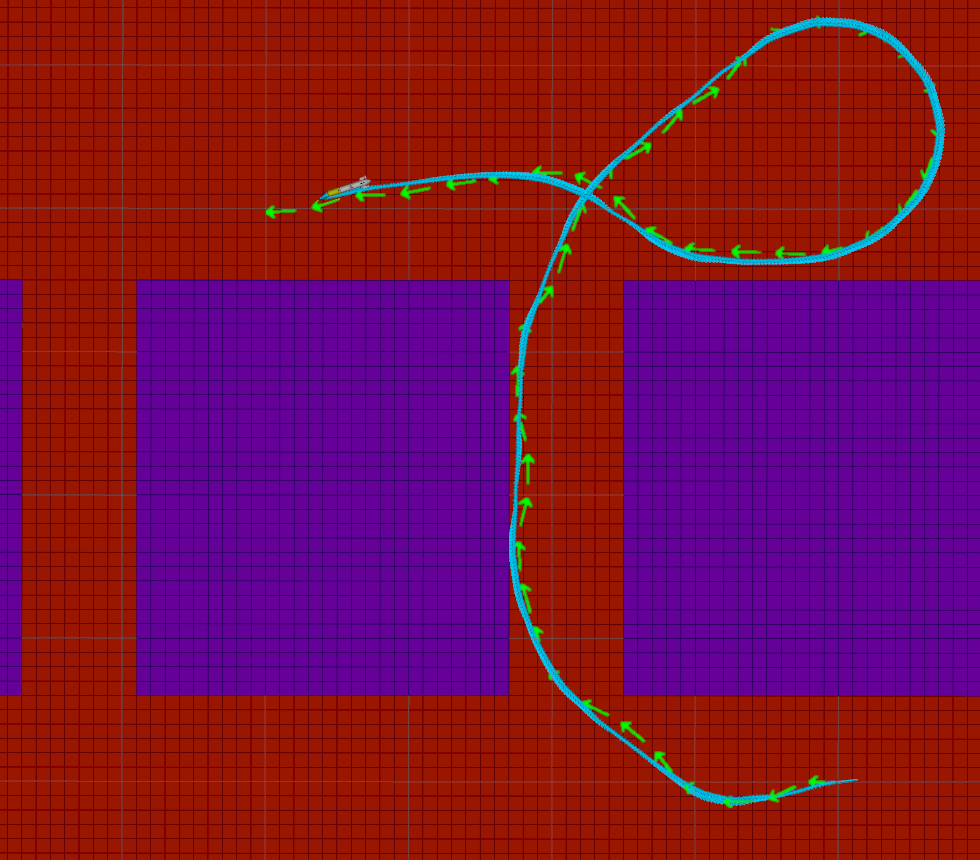
\includegraphics[width=.45\linewidth]{PlannKinodRRTQ1Miss}} \quad
%     \subfloat[Query 2]
%     {\label{fig:PlannKinodRRTQ2Miss}%
%      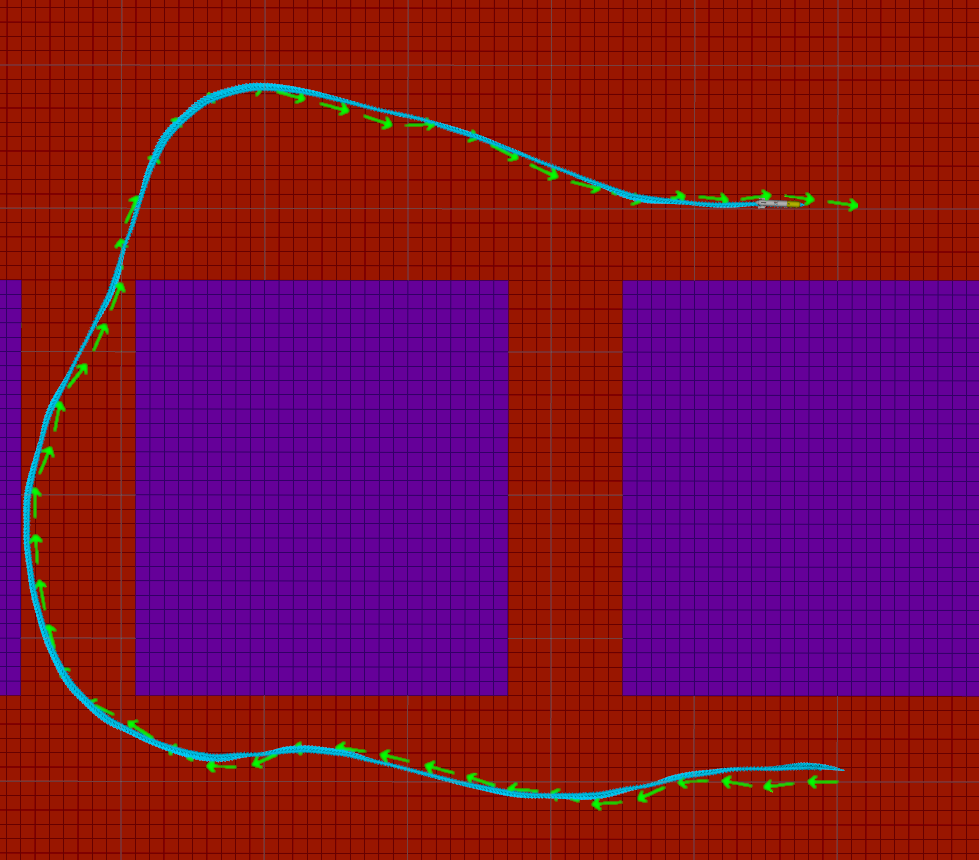
\includegraphics[width=.45\linewidth]{PlannKinodRRTQ2Miss}}
% \caption[Simulation of the Sparus~II AUV attempting to follow a solution path
% calculated by an RRT under motion constraints.]
% {Simulated environment composed of obstacles that create narrow passages.
% Two different start-to-goal query solutions that were calculated by an \ac{RRT}
% algorithm under motion constraints are shown in green. A simulated Sparus~II
% \ac{AUV} followed the paths. In this case, the \ac{RRT} algorithm does
% not provide any guarantee for optimality.}
% \label{fig:PlannKinodRRTQueries}
% \end{figure}

The second alternative uses the \ac{RRT*} algorithm and the Dubins curves, which
work as a steering function equivalent to Eq.~\eqref{eq:KinEqAUV2D}.
Figures~\ref{fig:PlannDubinsRRTstarQ1Miss}
and~\ref{fig:PlannDubinsRRTstarQ2Miss} depict how, with this approach, the
simulated Sparus~II \ac{AUV} follows (near) optimal paths of minimal length.
Although this latter approach generates better and more feasible solution paths,
there are also some risky states; these were generated because the planner tried to
provide the shortest paths, which were close to nearby obstacles. This
specific issue about the safety of the resulting path is addressed in detail in
Chapter~\ref{ch:plann_online}.

% \begin{figure}[htbp]
%     \myfloatalign
% %     \subfloat[\ldots.]
% %     {\label{fig:PlannKinodRRTQ1Sol}
% %     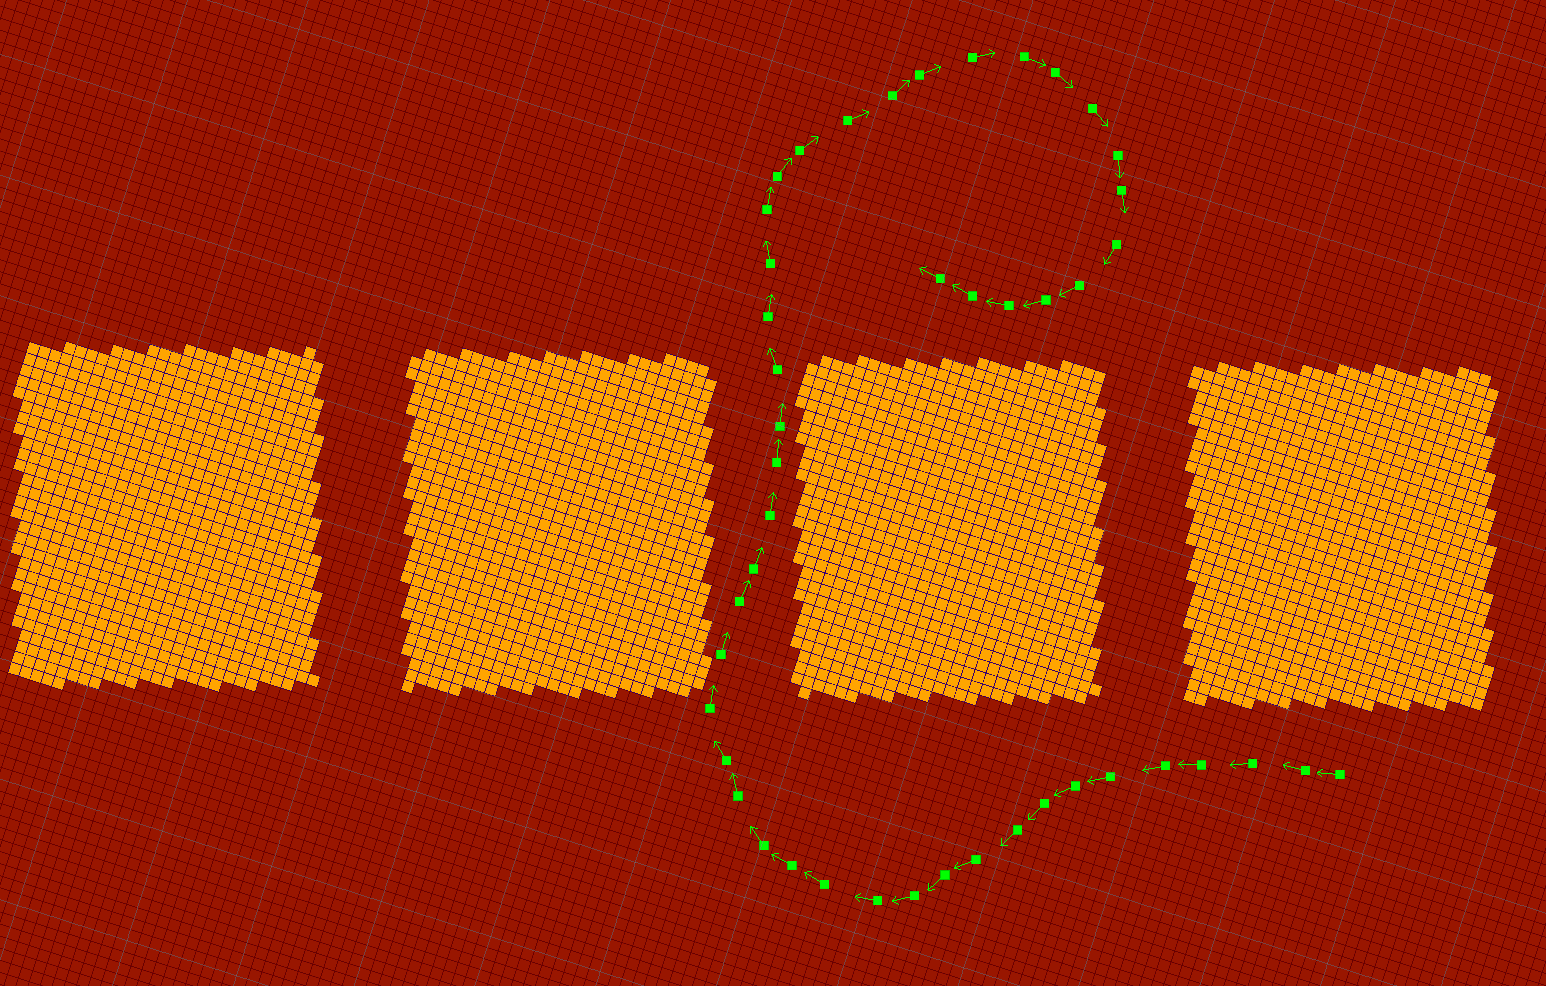
\includegraphics[width=.45\linewidth]{PlannKinodRRTQ1Sol}} \quad
% %     \subfloat[\ldots]
% %     {\label{fig:PlannKinodRRTQ2Sol}%
% %      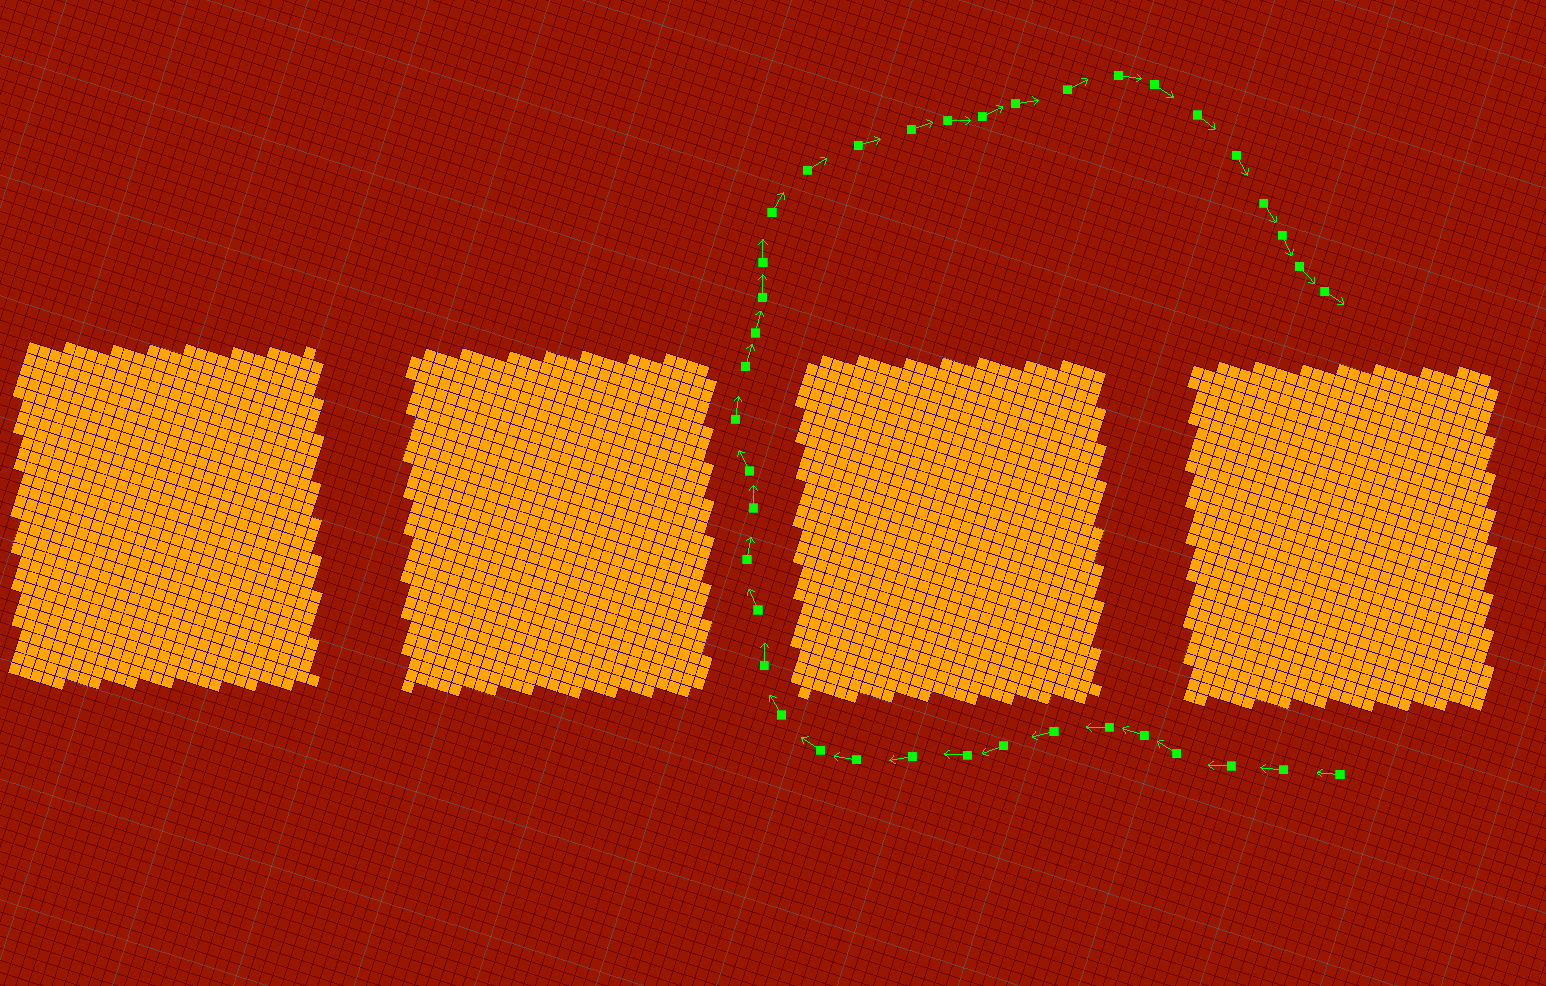
\includegraphics[width=.45\linewidth]{PlannKinodRRTQ2Sol}}\\
%     \subfloat[Query 1]
%     {\label{fig:PlannDubinsRRTstarQ1Miss}
%     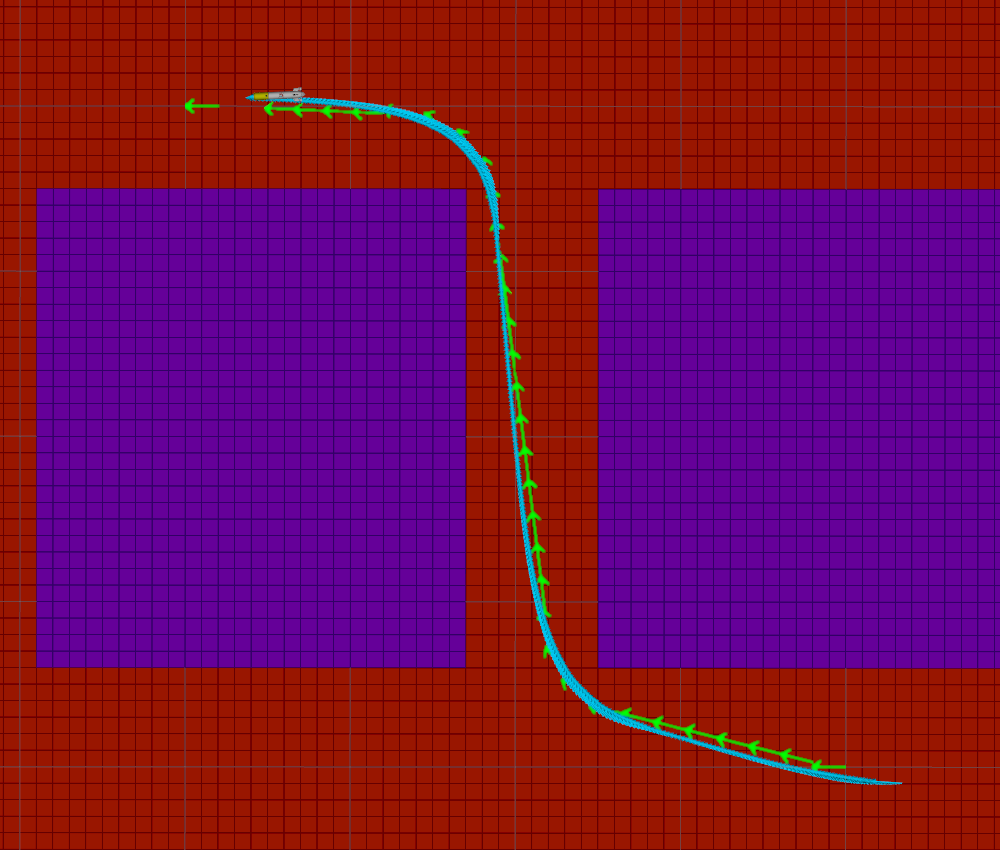
\includegraphics[width=.45\linewidth]{PlannDubinsRRTstarQ1Miss}} \quad
%     \subfloat[Query 2]
%     {\label{fig:PlannDubinsRRTstarQ2Miss}%
%      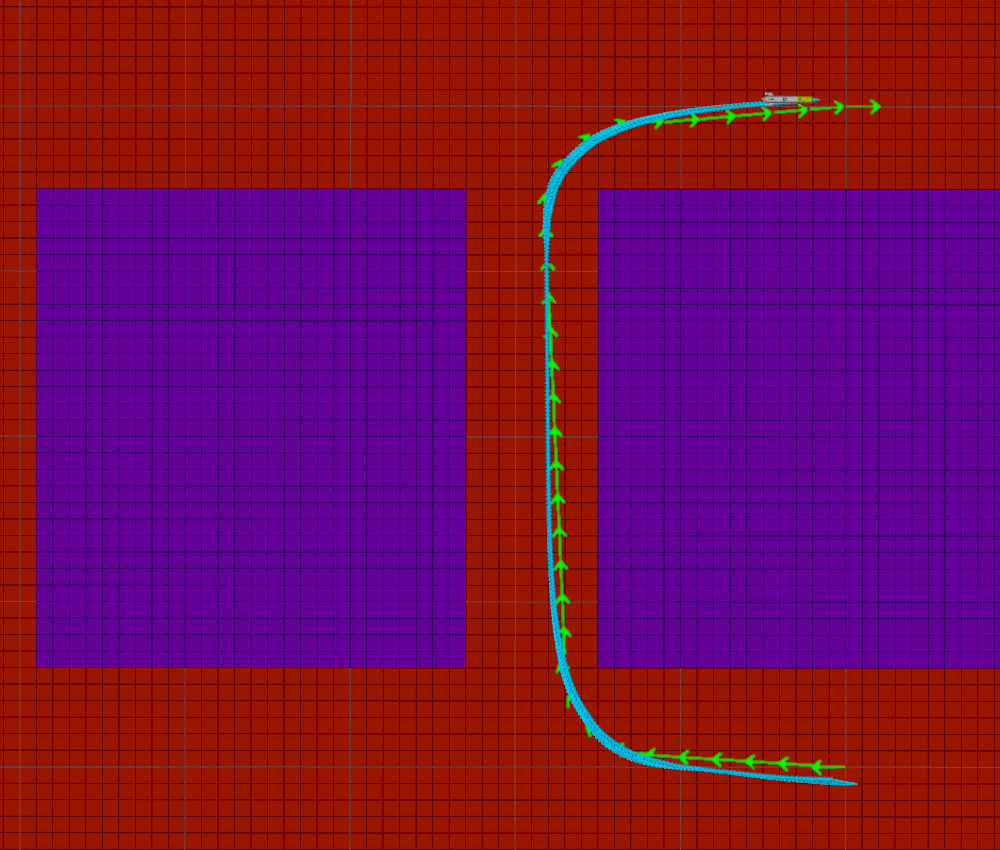
\includegraphics[width=.45\linewidth]{PlannDubinsRRTstarQ2Miss}}
% \caption[Simulation of the Sparus~II AUV attempting to follow a solution path
% calculated by an RRT* algorithm with Dubins curves as steering function.]
% {Simulated environment composed of two obstacles that create a narrow passage.
% Two different start-to-goal query solutions that were calculated by an \ac{RRT*}
% algorithm with Dubins curves as steering function are shown in green. A simulated
% Sparus~II \ac{AUV} followed the near optimal paths.}
% \label{fig:PlannDubinsRRTstarQueries}
% \end{figure}

A final remark about the content of this chapter is the fact that all cases
assume an \ac{AUV} that navigates at a constant depth. Even though this
assumption is valid in several applications, there are others, however, that
require to vary the vertical position of the vehicle. For this reason, the next
chapter covers the extension of this latter approach (using Dubins curves) for
dealing with \ac{3D} workspaces.

% \subsubsection{Non Optimal Motions using the RRT}
% \subsubsection{Optimal Motions using the RRT*}

% ---------------------------------------------------------------------------
%: ----------------------- end of thesis sub-document ------------------------
% ---------------------------------------------------------------------------

